%=======================================================================
%  Blockchain-Based Electronic Voting: Modelling and Experimental
%  Evaluation of Bribery, Sybil and Ballot-Stuffing Attacks
%
%  Every numeric value in this document is injected from the
%  experimental output by generate_report.py (generated/numbers.tex);
%  no result is typed in by hand. Compile with:
%      python generate_report.py
%=======================================================================
\documentclass[11pt,a4paper]{article}

\usepackage[T1]{fontenc}
\usepackage[utf8]{inputenc}
\usepackage{mathptmx}                      % Times text + math
\usepackage[scaled=0.88]{helvet}           % Helvetica for headings
\usepackage{amsmath,amssymb}
\usepackage[margin=2.6cm,top=2.8cm,bottom=2.9cm]{geometry}
\usepackage{graphicx}
\usepackage{booktabs}
\usepackage{tabularx}
\usepackage{longtable}
\usepackage{multirow}
\usepackage{float}
\usepackage{xcolor}
\usepackage{enumitem}
\usepackage{microtype}
\usepackage{setspace}
\usepackage{fancyhdr}
\usepackage{titlesec}
\usepackage[font=small,labelfont=bf,labelsep=period,justification=justified]{caption}
\usepackage{tcolorbox}
\usepackage{url}
\usepackage[hidelinks]{hyperref}

%--- palette (matches the figure palette in visualisation/style.py) ----
\definecolor{accent}{HTML}{0072B2}
\definecolor{warm}{HTML}{D55E00}
\definecolor{inkmuted}{HTML}{4D4D4D}
\definecolor{rule}{HTML}{BFBFBF}
\definecolor{panel}{HTML}{F4F7FA}

\hypersetup{colorlinks=true, linkcolor=accent, citecolor=accent,
            urlcolor=accent, linktoc=all,
            pdftitle={Blockchain-Based Electronic Voting: Modelling and
                      Experimental Evaluation of Bribery, Sybil and
                      Ballot-Stuffing Attacks},
            pdfsubject={MSc Computing Science dissertation}}

%--- headings ----------------------------------------------------------
\titleformat{\section}{\normalfont\sffamily\large\bfseries\color{black}}
            {\thesection}{0.8em}{}[\vspace{2pt}\color{rule}\hrule height 0.6pt]
\titleformat{\subsection}{\normalfont\sffamily\normalsize\bfseries}{\thesubsection}{0.7em}{}
\titleformat{\subsubsection}{\normalfont\sffamily\small\bfseries}{\thesubsubsection}{0.6em}{}
\titlespacing*{\section}{0pt}{20pt}{10pt}
\titlespacing*{\subsection}{0pt}{14pt}{6pt}

\pagestyle{fancy}
\fancyhf{}
\renewcommand{\headrulewidth}{0.4pt}
\fancyhead[L]{\footnotesize\sffamily\color{inkmuted}Blockchain-Based E-Voting: Attack Modelling and Evaluation}
\fancyhead[R]{\footnotesize\sffamily\color{inkmuted}\thepage}

\setlength{\parskip}{0.42em}
\setlength{\parindent}{0pt}
\onehalfspacing

%--- callout box -------------------------------------------------------
\newtcolorbox{finding}[1][]{colback=panel, colframe=accent, boxrule=0pt,
  leftrule=2.6pt, arc=1pt, left=9pt, right=9pt, top=7pt, bottom=7pt,
  fontupper=\normalsize, #1}

\newcommand{\finhead}[1]{\textsf{\bfseries #1}\par\vspace{2pt}}

%--- shorthands --------------------------------------------------------
\newcommand{\Prob}{\mathbb{P}}
\newcommand{\Ex}{\mathbb{E}}
\newcommand{\Bin}{\mathrm{Binomial}}
\newcommand{\Uv}{U_{v}}
\newcommand{\figref}[1]{Figure~\ref{#1}}
\newcommand{\tabref}[1]{Table~\ref{#1}}
\newcommand{\eqnref}[1]{Equation~(\ref{#1})}
\newcommand{\code}[1]{\texttt{\small #1}}

%--- generated numbers -------------------------------------------------
% Generated by generate_report.py -- do not edit by hand.
% Every value here is read from results/ output.

\newcommand{\BallotCeilingPct}{30}
\newcommand{\BallotCostRatio}{15}
\newcommand{\BallotStuffingAbsReduction}{0.325}
\newcommand{\BallotStuffingAcceptedBaseline}{0.498}
\newcommand{\BallotStuffingAcceptedProtected}{0.253}
\newcommand{\BallotStuffingBaseline}{0.442}
\newcommand{\BallotStuffingBaselineMedian}{0.0000}
\newcommand{\BallotStuffingBaselineStd}{0.487}
\newcommand{\BallotStuffingCIHigh}{0.343}
\newcommand{\BallotStuffingCILow}{0.308}
\newcommand{\BallotStuffingChernoffGap}{0.0216}
\newcommand{\BallotStuffingChernoffHolds}{100.0}
\newcommand{\BallotStuffingChernoffValid}{3,604}
\newcommand{\BallotStuffingIntervalWidth}{0.043}
\newcommand{\BallotStuffingMCError}{3.94e-4}
\newcommand{\BallotStuffingMCMaxError}{0.0230}
\newcommand{\BallotStuffingProtected}{0.116}
\newcommand{\BallotStuffingRelReduction}{73.7}
\newcommand{\BestPureMax}{0.423}
\newcommand{\BestPureMeanBaseline}{0.277}
\newcommand{\BestPureMin}{0.316}
\newcommand{\BestPureViableCount}{4}
\newcommand{\BriberyAbsReduction}{0.287}
\newcommand{\BriberyBaseline}{0.350}
\newcommand{\BriberyBaselineMedian}{0.0000}
\newcommand{\BriberyBaselineStd}{0.474}
\newcommand{\BriberyCIHigh}{0.304}
\newcommand{\BriberyCILow}{0.269}
\newcommand{\BriberyChernoffGap}{0.0423}
\newcommand{\BriberyChernoffHolds}{100.0}
\newcommand{\BriberyChernoffValid}{1,088}
\newcommand{\BriberyIntervalWidth}{0.018}
\newcommand{\BriberyMCError}{7.98e-5}
\newcommand{\BriberyMCMaxError}{0.0149}
\newcommand{\BriberyProtected}{0.064}
\newcommand{\BriberyRelReduction}{81.9}
\newcommand{\CertificationEpsilon}{10^{-3}}
\newcommand{\ChainIntegrityHeld}{never violated}
\newcommand{\CoalitionBetterCount}{4}
\newcommand{\CoalitionMeanBaseline}{0.800}
\newcommand{\CoalitionMeanGain}{0.522}
\newcommand{\CoalitionMeanProtected}{0.000}
\newcommand{\CoalitionScenarioCount}{5}
\newcommand{\ConvergenceFinalError}{0.0018}
\newcommand{\ConvergenceMaxSize}{50,000}
\newcommand{\ConvergenceMinSize}{10}
\newcommand{\ConvergenceSettles}{3,000}
\newcommand{\ConvergenceTolerance}{0.01}
\newcommand{\CriticalDetectionBindingCount}{4}
\newcommand{\CriticalDetectionMax}{0.118}
\newcommand{\CriticalDetectionMin}{0.050}
\newcommand{\ElectionTrials}{300}
\newcommand{\ElectorateMax}{4,999}
\newcommand{\ElectorateMin}{200}
\newcommand{\FigureCount}{10}
\newcommand{\FlipBallotStuffingBaseline}{55.0}
\newcommand{\FlipBallotStuffingProtected}{8.3}
\newcommand{\FlipBallotStuffingRelReduction}{84.8}
\newcommand{\FlipBriberyBaseline}{44.0}
\newcommand{\FlipBriberyProtected}{1.3}
\newcommand{\FlipBriberyRelReduction}{97.0}
\newcommand{\FlipSybilBaseline}{54.7}
\newcommand{\FlipSybilProtected}{11.3}
\newcommand{\FlipSybilRelReduction}{79.3}
\newcommand{\GateOpenBaseline}{5}
\newcommand{\GateOpenProtected}{0}
\newcommand{\IdentityCostRatio}{40}
\newcommand{\LowerTailShareMax}{30.6}
\newcommand{\LowerTailShareMin}{20.6}
\newcommand{\MonteCarloTrials}{2,000}
\newcommand{\MostResilient}{sybil}
\newcommand{\ProtectedQ}{0.55}
\newcommand{\ProtectionHeadroom}{4.7}
\newcommand{\RuntimeSeconds}{7.9}
\newcommand{\SFiveBStar}{57,100}
\newcommand{\SFiveBudget}{8,000}
\newcommand{\SFiveExactFlip}{0.000}
\newcommand{\SFiveM}{550}
\newcommand{\SFiveMReachable}{76}
\newcommand{\SFiveN}{5,000}
\newcommand{\SFiveQCritical}{0.000}
\newcommand{\SFiveQVoter}{0.167}
\newcommand{\SFiveTStar}{0}
\newcommand{\SFourBStar}{499,400}
\newcommand{\SFourBudget}{5,000,000}
\newcommand{\SFourExactFlip}{0.316}
\newcommand{\SFourM}{4,758}
\newcommand{\SFourMReachable}{4,750}
\newcommand{\SFourN}{5,000}
\newcommand{\SFourQCritical}{0.051}
\newcommand{\SFourQVoter}{0.167}
\newcommand{\SFourTStar}{5,000}
\newcommand{\SOneBStar}{2,880}
\newcommand{\SOneBriberyPFull}{0.423}
\newcommand{\SOneBudget}{3,000}
\newcommand{\SOneExactFlip}{0.423}
\newcommand{\SOneM}{35}
\newcommand{\SOneMReachable}{34}
\newcommand{\SOneN}{100}
\newcommand{\SOneQCritical}{0.118}
\newcommand{\SOneQVoter}{0.118}
\newcommand{\SOneTStar}{37}
\newcommand{\SThreeBStar}{2,998,650}
\newcommand{\SThreeBallotPFull}{0.085}
\newcommand{\SThreeBudget}{3,000,000}
\newcommand{\SThreeExactFlip}{0.320}
\newcommand{\SThreeM}{19,015}
\newcommand{\SThreeMCertified}{19,515}
\newcommand{\SThreeMReachable}{19,000}
\newcommand{\SThreeN}{100,000}
\newcommand{\SThreeQCritical}{0.050}
\newcommand{\SThreeQVoter}{0.111}
\newcommand{\SThreeTStar}{20,000}
\newcommand{\STwoBStar}{249,480}
\newcommand{\STwoBudget}{250,000}
\newcommand{\STwoExactFlip}{0.328}
\newcommand{\STwoM}{1,943}
\newcommand{\STwoMReachable}{1,937}
\newcommand{\STwoN}{10,000}
\newcommand{\STwoQCritical}{0.072}
\newcommand{\STwoQVoter}{0.118}
\newcommand{\STwoTStar}{2,083}
\newcommand{\ScaleBallotLarge}{0.000}
\newcommand{\ScaleBallotSmall}{0.237}
\newcommand{\ScaleBriberyLarge}{0.000}
\newcommand{\ScaleBriberySmall}{1.000}
\newcommand{\ScaleSybilLarge}{0.702}
\newcommand{\ScaleSybilSmall}{0.623}
\newcommand{\Seed}{42}
\newcommand{\SensitivityAtLeastAsGood}{100}
\newcommand{\SensitivityConfigs}{108}
\newcommand{\SensitivityStrictlyBetter}{100}
\newcommand{\SybilAbsReduction}{0.345}
\newcommand{\SybilAcceptedBaseline}{0.537}
\newcommand{\SybilAcceptedProtected}{0.299}
\newcommand{\SybilBaseline}{0.480}
\newcommand{\SybilBaselineMedian}{0.0593}
\newcommand{\SybilBaselineStd}{0.492}
\newcommand{\SybilCIHigh}{0.362}
\newcommand{\SybilCILow}{0.327}
\newcommand{\SybilCeilingPct}{20}
\newcommand{\SybilChernoffGap}{0.0260}
\newcommand{\SybilChernoffHolds}{100.0}
\newcommand{\SybilChernoffValid}{3,471}
\newcommand{\SybilIntervalWidth}{0.044}
\newcommand{\SybilMCError}{3.95e-4}
\newcommand{\SybilMCMaxError}{0.0305}
\newcommand{\SybilProtected}{0.136}
\newcommand{\SybilRelReduction}{71.8}
\newcommand{\TestCount}{122}
\newcommand{\TotalTrials}{2,500}
\newcommand{\VoterIndifferenceMax}{0.167}
\newcommand{\VoterIndifferenceMin}{0.111}
\newcommand{\WEA}{104}
\newcommand{\WEB}{122,592}
\newcommand{\WEN}{4,458}
\newcommand{\WEP}{1051.88}
\newcommand{\WER}{372.81}
\newcommand{\WES}{981}
\newcommand{\WET}{328}
\newcommand{\WEUvBase}{45.85}
\newcommand{\WEUvProt}{-364.10}
\newcommand{\WEballotPBase}{0.000}
\newcommand{\WEballotPProt}{0.000}
\newcommand{\WEballotmuBase}{59.1}
\newcommand{\WEballotmuProt}{27.2}
\newcommand{\WEchernoffBase}{0.875}
\newcommand{\WEchernoffProt}{not applicable}
\newcommand{\WEdecisionBase}{accept}
\newcommand{\WEdecisionProt}{reject}
\newcommand{\WEexactBase}{0.153}
\newcommand{\WEexactProt}{0.000}
\newcommand{\WEm}{261}
\newcommand{\WEmcBase}{0.160}
\newcommand{\WEmcProt}{0.000}
\newcommand{\WEmuBase}{252.7}
\newcommand{\WEmuProt}{0.0}
\newcommand{\WEpbBase}{0.036}
\newcommand{\WEpbProt}{0.281}
\newcommand{\WEpdBase}{0.274}
\newcommand{\WEpdProt}{0.705}
\newcommand{\WEpsurviveBase}{0.771}
\newcommand{\WEpsurviveProt}{0.483}
\newcommand{\WEqBase}{0.229}
\newcommand{\WEqProt}{0.517}
\newcommand{\WEqbBase}{0.589}
\newcommand{\WEqbProt}{0.364}
\newcommand{\WEqsBase}{0.771}
\newcommand{\WEqsProt}{0.425}
\newcommand{\WEsybilPBase}{1.000}
\newcommand{\WEsybilPProt}{0.000}
\newcommand{\WEsybilmuBase}{549.3}
\newcommand{\WEsybilmuProt}{122.8}
\newcommand{\WEtrial}{79}

\graphicspath{{../results/plots/}}

\begin{document}

%=======================================================================
\begin{titlepage}
\thispagestyle{empty}
\centering
\vspace*{1.2cm}

{\sffamily\Large University of Glasgow}\\[2pt]
{\sffamily\normalsize School of Computing Science}\\[3.2cm]

{\color{rule}\rule{\textwidth}{0.9pt}}\\[0.7cm]
{\sffamily\LARGE\bfseries Blockchain-Based Electronic Voting}\\[0.42cm]
{\sffamily\Large Mathematical Modelling and Experimental Evaluation of}\\[0.18cm]
{\sffamily\Large Bribery, Sybil and Ballot-Stuffing Attacks}\\[0.7cm]
{\color{rule}\rule{\textwidth}{0.9pt}}\\[1.5cm]

{\large A game-theoretic and probabilistic security evaluation,}\\[3pt]
{\large with exact binomial analysis, Chernoff bounds and}\\[3pt]
{\large critical-threshold identification}\\[2.6cm]

{\sffamily\large MSc Computing Science}\\[0.35cm]
{\sffamily\normalsize Dissertation}\\[2.4cm]

\begin{minipage}{0.8\textwidth}
\centering
{\itshape Author, supervisor and submission date to be completed by the candidate.}
\end{minipage}

\vfill
{\footnotesize\color{inkmuted}
All results in this document are generated from the accompanying simulation code
(seed \Seed, \TotalTrials{} paired trials per vector) and are reproducible bit-for-bit.
No real election system, voter record or personal datum is used anywhere in this work.}
\end{titlepage}

%=======================================================================
\clearpage
\section*{Abstract}
\addcontentsline{toc}{section}{Abstract}

Electronic voting systems built on blockchain ledgers are frequently claimed to be
tamper-proof, but immutability of a recorded ballot is a different property from
resistance to the manipulation that occurs \emph{before} a ballot is recorded. This
dissertation asks a narrower and more answerable question: given a rational attacker
with a finite budget, how likely is manipulation to change an election outcome, and
what level of countermeasure is actually required to stop it?

Three manipulation vectors are modelled probabilistically and game-theoretically ---
bribery of genuine voters, Sybil registration of forged identities, and ballot
stuffing. Each is expressed as a sequence of independent Bernoulli attempts whose
outcome count follows a binomial distribution, with attack success defined as reaching
a manipulation threshold $m$: exactly the number of fraudulent votes needed to overturn
the election. Success probabilities are computed three ways --- exactly by the binomial
survival function, empirically by Monte Carlo simulation, and analytically by a
multiplicative Chernoff bound --- and the three are cross-validated against one another.

The evaluation runs \TotalTrials{} paired randomised trials per vector, comparing a
baseline configuration against a protected configuration in which a blockchain-backed
audit ledger is combined with digital signatures, identity verification and ballot
validation. It is those validation and detection controls, not the ledger, that raise
detection and lower acceptance; the ledger contributes integrity, immutability and
auditability, and the experiment is designed to keep the two contributions
distinguishable. The same underlying scenario is used for both arms of each pair,
so the comparison is a matched design rather than two independent samples. A concrete
layer complements the statistics: \ElectionTrials{} elections are genuinely mined on a
proof-of-work chain and attacked, so that abstract success probabilities are tied to
actual winner flips.

The protected configuration reduces mean success probability by \BriberyRelReduction\%
for bribery, \SybilRelReduction\% for Sybil attacks and \BallotStuffingRelReduction\%
for ballot stuffing, and reduces real winner-flip rates from \FlipBriberyBaseline\%,
\FlipSybilBaseline\% and \FlipBallotStuffingBaseline\% to \FlipBriberyProtected\%,
\FlipSybilProtected\% and \FlipBallotStuffingProtected\% respectively. Chain integrity
was \ChainIntegrityHeld{} across all trials.

Beyond these aggregate results the dissertation contributes two extensions. First, a
set of \emph{critical-threshold solvers} inverts the model: rather than reporting how
likely an attack is, they report the parameter value at which it stops being viable.
The most consequential of these is the critical detection probability $q_d^*$, which
lies between \CriticalDetectionMin{} and \CriticalDetectionMax{} across the
\CriticalDetectionBindingCount{} of \CoalitionScenarioCount{} benchmark scenarios where
detection is the binding constraint --- between four and eleven times weaker than the
detection the protected configuration actually delivers, and in the fifth scenario the
attack never pays at any detection level. Deterrence, on this model,
is far cheaper than prevention. Second, a \emph{coalition} model allows one attacker
to split a single budget across all three vectors at once. The exact distribution of
the combined attack is obtained by convolution rather than approximation, and the
mixed strategy strictly outperforms the best single-vector strategy in
\CoalitionBetterCount{} of \CoalitionScenarioCount{} scenarios, raising mean success
probability from \BestPureMeanBaseline{} to \CoalitionMeanBaseline{}. Single-vector
security analysis therefore understates the risk, while the modelled countermeasures
reduce the coalition attack to the same degree as they reduce each vector alone across
the benchmark scenarios examined.

\vspace{0.6em}
\noindent\textbf{Keywords:} electronic voting, blockchain, bribery, Sybil attack,
ballot stuffing, game theory, Chernoff bound, binomial analysis, security thresholds.

%=======================================================================
\clearpage
\tableofcontents
\clearpage
\listoffigures
\listoftables
\clearpage

%=======================================================================
\section{Introduction}

\subsection{Motivation}

The appeal of a blockchain-backed ballot box is easy to state: once a vote is written
to an append-only, hash-linked ledger and replicated across independent nodes, altering
it after the fact is computationally infeasible and, more importantly, immediately
visible. That property is real, and the implementation accompanying this dissertation
demonstrates it directly --- a vote modified after mining is caught by chain validation,
with the exact offending block index reported.

The property is also narrower than it is usually made to sound. Immutability protects a
vote \emph{after} it is recorded. It says nothing about whether the vote should have
existed at all. A ballot cast by a voter who was paid to vote a particular way is
recorded just as faithfully as an honest one; so is a ballot cast by a forged identity
that passed registration, and so is a ballot injected by an attacker with system access.
In each case the ledger is perfectly consistent and the election is still wrong. The
security question that matters, then, is not whether the record can be altered, but how
much manipulation an attacker can push through the front door, and what it costs them.

That reframing makes the problem quantitative. An attacker has a budget, faces a per
attempt cost, and succeeds only if enough fraudulent votes survive the system's
defences to overturn the margin. Each of those quantities is a number, and the
relationship between them is a probability distribution rather than a binary
vulnerability. This dissertation takes that view seriously and works it through.

\subsection{Research questions}

\begin{enumerate}[label=\textbf{RQ\arabic*.},leftmargin=2.6em,itemsep=3pt]
  \item How does the probability that an attack overturns an election outcome depend on
        the attacker's budget, the per-attempt cost, and the system's detection
        capability?
  \item How accurately do a Monte Carlo estimate and a Chernoff upper bound reproduce
        the exact binomial probability, and where does each remain useful at scale?
  \item How much does the protected configuration --- a blockchain-backed
        audit ledger \emph{combined with} digital signatures, identity
        verification and ballot validation --- reduce attack success,
        measured as a matched comparison on identical scenarios?
  \item What is the \emph{minimum} countermeasure strength that makes each attack
        non-viable, as opposed to merely less likely to succeed?
  \item Does an attacker who combines all three vectors against a single budget
        outperform one who commits to the best single vector, and does that change the
        security conclusion?
\end{enumerate}

RQ1--RQ3 are the descriptive questions the base model answers. RQ4 and RQ5 are this
dissertation's extensions and are, in the author's view, the more useful pair: a
defender cannot act on a probability curve, but can act on a threshold.

\subsection{Contributions}

\begin{enumerate}[leftmargin=1.6em,itemsep=3pt]
  \item A complete probabilistic model of three e-voting manipulation vectors
        (Section~\ref{sec:model}), implemented with exact binomial computation,
        Monte Carlo simulation and correctly-signed Chernoff bounds in both tails,
        with each equation traceable to its implementing function.
  \item A matched experimental evaluation over \TotalTrials{} paired randomised trials
        per vector (Section~\ref{sec:findings}), reporting bootstrap confidence
        intervals rather than point estimates alone.
  \item A concrete validation layer in which \ElectionTrials{} elections are actually
        mined on a proof-of-work chain and attacked, tying every abstract probability
        to a real winner flip (Section~\ref{sec:findings-concrete}).
  \item Seven \emph{critical-threshold solvers} (Section~\ref{sec:thresholds}) that
        invert the model and return the parameter value at which an attack ceases to be
        viable, including the break-even attacker budget and the critical detection
        probability.
  \item A \emph{coalition attack} model (Section~\ref{sec:coalition}) in which one
        budget is split across all three vectors, with the combined distribution
        evaluated exactly by convolution, plus a robustness sweep over
        \SensitivityConfigs{} cost and capacity configurations.
\end{enumerate}

\subsection{Scope, and what this work is not}

This is a simulation study with synthetic data. It models no real election, no real
voter, and no real deployed system; the candidates are labelled \emph{A} and \emph{B}
and have no referent. The blockchain component is a working but educational
proof-of-work implementation, not a distributed consensus network with real nodes,
network partitions or economic security. Countermeasures are modelled as probability
parameters rather than as specific cryptographic constructions: the model says what
happens if identity verification catches a forged registration with probability $p_d$,
not how such verification is built.

The work is also deliberately confined to manipulation of vote \emph{inputs}. Attacks on
the consensus layer itself --- majority hash-power attacks, chain reorganisation, eclipse
attacks --- are out of scope, as are coercion and receipt-freeness, which raise questions
of ballot secrecy rather than of ballot count. Section~\ref{sec:limitations} returns to
these boundaries and to what would be needed to cross them.

%=======================================================================
%=======================================================================
%  Literature Review
%=======================================================================
\section{Literature Review}
\label{sec:litreview}

\subsection{Scope and method of the review}

This review covers four bodies of work that the dissertation draws
together, and it is organised by the question each body answers rather
than chronologically.

\begin{enumerate}[leftmargin=1.6em,itemsep=2pt]
  \item \textbf{What has been built, and what is claimed for it?}
        Electronic and blockchain-based voting systems, from
        cryptographic verifiable-voting schemes to ledger-backed
        proposals (Sections~\ref{sec:lit-evoting}--\ref{sec:lit-bcvoting}).
  \item \textbf{What breaks when it is deployed?} The empirical
        security literature: analyses of fielded internet-voting systems
        and the critical response to blockchain voting specifically
        (Section~\ref{sec:lit-critique}).
  \item \textbf{How is manipulation modelled formally?} Bribery as a
        computational problem, coercion and receipt-freeness, Sybil
        identity attacks, and the statistical forensics of fraudulent
        tallies (Sections~\ref{sec:lit-bribery}--\ref{sec:lit-forensics}).
  \item \textbf{What tools exist for reasoning about a rational,
        resource-bounded attacker?} Concentration inequalities and
        game-theoretic security analysis
        (Section~\ref{sec:lit-probgame}).
\end{enumerate}

Sources were located by targeted search of the primary security venues
(USENIX Security, ACM CCS, Financial Cryptography, IEEE S\&P and their
workshops), the artificial-intelligence and economics literature for
the manipulation-theory strand, and two recent systematic reviews of
blockchain voting~\cite{ohize2025,rahul2025} used as entry points into
the applied literature. Priority was given to peer-reviewed primary
sources; where a widely-cited result exists only as a technical report
or research blog post, as with the Dark DAO
construction~\cite{daian2018}, this is stated explicitly rather than
disguised by citation formatting.

Section~\ref{sec:lit-synthesis} closes the review by identifying what
the four bodies of work leave unaddressed, which is the gap this
dissertation occupies.

\subsection{Electronic voting before blockchain}
\label{sec:lit-evoting}

The security requirements for an electronic election were substantially
settled before distributed ledgers entered the conversation, and it is
worth restating them because blockchain proposals are frequently
evaluated against a narrower list.

\textbf{Verifiability.} A voter should be able to confirm that their
ballot was recorded as cast, and any observer should be able to confirm
that the recorded ballots were tallied correctly. Adida's
Helios~\cite{adida2008} is the canonical open-audit implementation: it
publishes encrypted ballots to a public bulletin board and proves the
tally correct with homomorphic encryption and zero-knowledge proofs, so
that correctness rests on mathematics rather than on trusting the
election authority. Helios matters to the present work as a
counterexample to a common framing: it delivers public verifiability
with no ledger, no chain and no consensus mechanism, which shows that
the verifiability argument for blockchain voting is not an argument for
blockchain specifically.

\textbf{Ballot secrecy and its stronger forms.} Secrecy alone is
insufficient if a voter can \emph{prove} how they voted, because a
provable vote is a sellable vote. Benaloh and
Tuinstra~\cite{benaloh1994} formalised \emph{receipt-freeness}: the
requirement that a voter cannot construct a convincing proof of their
choice even if they want to. Juels, Catalano and
Jakobsson~\cite{juels2005} strengthened this to
\emph{coercion-resistance}, covering an adversary who can interact with
the voter during voting, demand credentials, or require abstention;
their scheme lets a coerced voter surrender a fake credential
indistinguishable from a real one.

This distinction sets the boundary of the present work. Bribery, as
modelled here, presupposes that the briber can verify compliance well
enough for the transaction to be worth making. A system that is
genuinely receipt-free undermines that presupposition at the root,
which is a different and stronger defence than the detection-based one
modelled in this dissertation. Section~\ref{sec:limitations} returns to
this.

\subsection{Blockchain-based voting proposals}
\label{sec:lit-bcvoting}

Nakamoto's chained proof-of-work construction~\cite{nakamoto2008}
supplied a mechanism with obvious surface appeal for elections: an
append-only, hash-linked, replicated log in which retrospective edits
invalidate every subsequent hash and are therefore detectable by anyone
holding a copy.

The most rigorous academic instantiation is McCorry, Shahandashti and
Hao's Open Vote Network~\cite{mccorry2017}, a boardroom-voting protocol
implemented as an Ethereum smart contract, which achieves maximum voter
privacy in the sense that a vote can only be revealed by full collusion
of all remaining participants, and which is self-tallying: no trusted
authority computes the result. It is a genuine cryptographic
contribution rather than a ledger with ballots written into it. Its
scope, however, is explicitly the boardroom --- tens of voters, all
known to one another --- and its cost and collusion properties do not
transfer to a public election.

The wider applied literature is large and, by the assessment of its own
systematic reviewers, uneven. Ohize et al.~\cite{ohize2025} survey
architectures and trends across the field and identify scalability,
post-quantum security, voter authentication, regulatory frameworks and
cross-chain interoperability as the persistent open problems. Rahul,
Gulia and Gill~\cite{rahul2025} review 55 journal articles and reach a
similar conclusion, noting that security, transparency and trust remain
unresolved worldwide rather than settled by any existing proposal. Two
observations from these reviews shape the present work. First,
\emph{voter authentication} is repeatedly named as an open problem,
which is precisely the Sybil vector modelled here. Second, the surveyed
proposals are overwhelmingly evaluated on functionality, throughput and
cryptographic properties rather than on quantified resistance to a
budgeted attacker --- the gap this dissertation addresses.

\subsection{The critical response: what happens on deployment}
\label{sec:lit-critique}

Against the proposal literature stands a smaller and considerably more
sobering body of empirical analysis.

Springall et al.~\cite{springall2014} examined Estonia's I-voting
system, the most established national internet-voting deployment, by
observing operations directly and reconstructing the system in the
laboratory. They reported serious procedural lapses and architectural
weaknesses sufficient, in their assessment, for a state-level attacker
to alter results undetectably, and recommended discontinuing the
system. The finding relevant here is not the specific vulnerabilities
but the location of them: the client platform and the operational
procedures surrounding the count, not the cryptography.

Specter, Koppel and Weitzner~\cite{specter2020} reverse-engineered
Voatz, the first internet-voting application used in U.S. federal
elections and marketed on its use of a blockchain. They found flaws
allowing an adversary to alter, stop or expose a voter's ballot, a
side-channel through which a passive network observer could recover the
secret ballot, and a dependence on third-party services with attendant
privacy exposure; West Virginia and a Washington county withdrew the
application from 2020 primaries following the analysis. The
architectural point is the important one: the blockchain sat behind an
application whose compromise made the ledger irrelevant, because votes
were corrupted before they reached it.

Park, Specter, Narula and Rivest~\cite{park2021} generalise these
observations into a direct argument that blockchain voting is worse
than internet voting rather than better. Their case is that blockchains
address a problem elections do not have --- disagreement about which
transactions occurred among mutually distrusting parties --- while
introducing new failure modes, and that the genuinely hard problems of
elections, namely software independence, secret ballots, voter
authentication and client-side integrity, are untouched. They further
note that a blockchain vote is a \emph{transparent} record, which is in
tension with ballot secrecy rather than supportive of it.

This dissertation adopts that critique as a premise to be tested
quantitatively rather than as a conclusion to be restated. The
experimental design deliberately grants the ledger everything its
proponents claim --- integrity is verified continuously and, as
Section~\ref{sec:findings} reports, was never violated in any trial ---
and then measures how many elections are stolen anyway.

\subsection{Bribery and vote buying as a formal problem}
\label{sec:lit-bribery}

Three distinct traditions model vote buying, and this dissertation
borrows from all three.

\textbf{Computational.} Faliszewski, Hemaspaandra and
Hemaspaandra~\cite{faliszewski2009} formalise bribery as a decision
problem: given per-voter prices and a budget, can the briber make a
preferred candidate win? They classify the complexity across voting
rules, establishing that some systems make optimal bribery
NP-hard --- complexity as a defensive barrier. The framing is
worst-case, combinatorial and deterministic: a bribed voter votes as
paid.

\textbf{Economic.} Becker's analysis of crime as a decision under
risk~\cite{becker1968} models an offender weighing gain against the
probability of detection multiplied by the penalty, and derives the
policy conclusion that deterrence can be achieved either by raising
detection or by raising penalties. Equation~(\ref{eq:m1}) in this
dissertation is exactly that calculation applied to a bribed voter, and
the critical-detection threshold of Section~\ref{sec:thresholds} is the
policy question in Becker's sense: how much detection is enough?

\textbf{Blockchain-specific.} Daian, Kell, Bentov and
Juels~\cite{daian2018} describe on-chain vote buying and the
\emph{Dark DAO}: a smart contract that pays for votes and enforces the
payment trustlessly, using trusted execution to verify compliance
without revealing the buyer. Their argument deserves emphasis in the
present context because it inverts the usual claim. A blockchain does
not merely fail to prevent vote buying; by making votes cryptographically
attributable and payments programmable and escrowed, it \emph{improves}
the market for votes, removing the counterparty risk that limits bribery
in traditional settings. This is a technical-report and research-blog
contribution rather than a peer-reviewed paper, and is cited as such,
but it is widely referenced and directly motivates treating bribery,
not tampering, as the primary threat to a ledger-based election.

The gap across all three: the computational tradition treats bribery
deterministically, the economic tradition treats the individual decision
without an electorate-level outcome model, and the blockchain-specific
work is a mechanism proposal rather than a quantified risk model. None
produces the quantity a defender needs --- the probability that a given
budget overturns a given margin against a given detection capability.

\subsection{Sybil attacks and identity}
\label{sec:lit-sybil}

Douceur~\cite{douceur2002} established that, absent a trusted
certification authority, a single entity in a distributed system can
present arbitrarily many distinct identities, and that no purely local
resource test reliably distinguishes them. For an election the
consequence is immediate and fatal: one-person-one-vote is the entire
premise, and a Sybil attack attacks the premise rather than the
mechanism.

Responses divide into those that reintroduce a trusted authority and
those that attempt to establish uniqueness without one. Borge et
al.~\cite{borge2017} propose proof-of-personhood, binding digital
identities to physical presence at pseudonym parties, explicitly to
recover one-per-person semantics in permissionless systems. The
approach illustrates both the necessity and the difficulty: physical
attendance is a strong Sybil barrier and an equally strong barrier to
accessibility, which is what electronic voting exists to improve.

This dissertation does not model any specific identity mechanism. It
parameterises the outcome instead --- a forged registration passes with
probability $q_s$ and is caught with probability $p_d$ --- which is
weaker than assuming a trusted authority and is deliberately
conservative. It also produces the finding, reported in
Section~\ref{sec:findings}, that identity verification rather than
ledger integrity is where the residual risk concentrates, consistent
with voter authentication being repeatedly flagged as an open problem in
the systematic reviews~\cite{ohize2025,rahul2025}.

\subsection{Ballot stuffing and statistical election forensics}
\label{sec:lit-forensics}

Ballot stuffing --- injecting fraudulent ballots not corresponding to
any voter --- is the least cryptographically interesting of the three
vectors and, historically, among the most common. The relevant
literature is statistical rather than cryptographic.

Klimek, Yegorov, Hanel and Thurner~\cite{klimek2012} show that
systematic irregularities leave detectable signatures in the joint
distribution of turnout and vote share across polling units: incremental
stuffing and extreme fraud produce characteristic distortions absent
from clean elections, and the authors identify these fingerprints in
several national elections. The methodological lesson carried into this
dissertation is that fraud is bounded by \emph{plausibility} as much as
by opportunity. An attacker who injects ballots without limit produces a
turnout figure that requires no probabilistic detection to notice. This
is the justification for the capacity ceilings imposed in the coalition
model (Section~\ref{sec:coalition-model}), which are otherwise a
modelling choice without grounding: they stand in for the anomaly
detection that election forensics performs.

\subsection{Probabilistic and game-theoretic security analysis}
\label{sec:lit-probgame}

The final strand supplies the analytical machinery.

\textbf{Concentration inequalities.} Chernoff's
bound~\cite{chernoff1952}, in the multiplicative form given by
Mitzenmacher and Upfal~\cite{mitzenmacher2017}, bounds the probability
that a sum of independent Bernoulli variables deviates from its mean,
and does so exponentially in the deviation. For this dissertation its
value is specific: it converts an empirical statement into a provable
one. A margin certified safe by the bound is safe irrespective of how
many simulation runs were performed, which is what makes the certified
margin of Section~\ref{sec:thresholds} a security claim rather than an
observation.

\textbf{Rational attackers.} Eyal and Sirer~\cite{eyal2014}
demonstrated with selfish mining that a blockchain protocol assumed
secure under an honest-majority model can be broken by a rational
minority that deviates profitably --- security depending on incentives,
not only on cryptography or on hash-power share. Liu et
al.~\cite{liu2019} survey the resulting body of game-theoretic
blockchain analysis, covering mining strategy, security games and
incentive design.

Two points transfer directly. First, the relevant question about an
attacker is what they would \emph{choose} to do, not what they are
capable of doing: Section~\ref{sec:thresholds-results} shows that a
budget-exhausting attacker performs strictly worse than a rational one,
so a defence tuned against maximum expenditure is tuned against the
wrong opponent. Second, deterrence is a legitimate security goal
distinct from prevention --- making an attack unprofitable is cheaper
than making it impossible, and the gap between those two thresholds is
quantified in this dissertation.

\subsection{Synthesis and research gap}
\label{sec:lit-synthesis}

\tabref{tab:gap} summarises what each strand supplies and what it
leaves open.

\begin{table}[htbp]
\centering
\caption{What the literature supplies, and what it leaves open.}
\label{tab:gap}
\small
\begin{tabular}{@{}p{3.5cm}p{5.1cm}p{5.1cm}@{}}
\toprule
\textbf{Strand} & \textbf{Supplies} & \textbf{Leaves open} \\
\midrule
Blockchain voting proposals
  \cite{mccorry2017,ohize2025,rahul2025}
& Architectures, cryptographic protocols, throughput evaluation
& No quantified success probability against a budgeted attacker \\
\addlinespace
Empirical critiques
  \cite{springall2014,specter2020,park2021}
& Evidence that deployments fail upstream of the ledger
& Qualitative argument; no model of how much manipulation gets through \\
\addlinespace
Bribery theory
  \cite{faliszewski2009,becker1968,daian2018}
& Complexity classification; the rational-offender calculus; on-chain vote-buying mechanisms
& Deterministic or individual-level; no electorate-scale outcome distribution \\
\addlinespace
Sybil and identity
  \cite{douceur2002,borge2017}
& Impossibility without trusted certification; countermeasure designs
& No probabilistic model of partial identity verification \\
\addlinespace
Election forensics
  \cite{klimek2012}
& Statistical signatures of stuffing; plausibility as a real constraint
& Detection after the fact, not a design threshold beforehand \\
\addlinespace
Probabilistic and game-theoretic tools
  \cite{chernoff1952,mitzenmacher2017,eyal2014,liu2019}
& Concentration bounds; rational-deviation analysis
& Not yet applied to e-voting manipulation as an integrated model \\
\bottomrule
\end{tabular}
\end{table}

Three gaps follow, and they define the contribution of this
dissertation.

\textbf{Gap 1: no quantified attacker model for e-voting
countermeasures.} The proposal literature evaluates systems on
cryptographic properties and performance; the critical literature
establishes qualitatively that deployments fail. Neither produces the
probability that a specific budget overturns a specific margin against
a specific detection capability. Sections~\ref{sec:model}
and~\ref{sec:findings} supply exactly that, over
\TotalTrials{} matched randomised trials per vector.

\textbf{Gap 2: probabilities are reported where thresholds are
needed.} A defender cannot act on a success-probability curve. The
inverse question --- what detection probability, what budget ceiling,
what margin makes this attack non-viable --- is not asked in the
e-voting literature, although Becker's economics of
deterrence~\cite{becker1968} and the game-theoretic blockchain
work~\cite{eyal2014,liu2019} both imply it should be.
Section~\ref{sec:thresholds} formulates seven such thresholds and
solves them.

\textbf{Gap 3: attack vectors are evaluated in isolation.} Every source
reviewed treats bribery, Sybil attacks and ballot stuffing separately.
No reviewed work models an attacker allocating one budget across
several vectors simultaneously. Section~\ref{sec:coalition} shows this
omission is not conservative: two of the three vectors are individually
infeasible in every benchmark scenario, yet their combination succeeds
decisively in four of five.


\section{Threat model and mathematical framework}
\label{sec:model}

\subsection{Threat model}

A single attacker attempts to change the outcome of a two-candidate election with $N$
enrolled voters. Let the honest tally leave the attacker's preferred candidate behind by
some margin; the \emph{manipulation threshold} $m$ is the number of additional
fraudulent votes needed to overturn that margin, so that

\begin{equation}
m = (\text{opponent votes} - \text{target votes}) + 1 ,
\label{eq:threshold}
\end{equation}

and the attack succeeds precisely when at least $m$ fraudulent votes survive every
countermeasure and reach the final count. Throughout this dissertation, ``attack
success'' means exactly this event and nothing weaker.

Three vectors are available.

\begin{description}[leftmargin=1.4em,style=nextline,itemsep=2pt]
  \item[Bribery.] The attacker offers a reward $R$ to genuine voters, constrained by a
    total budget $B$. A targeted voter accepts only if doing so is rationally
    incentivised. Each bribed vote is detected, and therefore discarded, with
    probability $q$.
  \item[Sybil registration.] The attacker submits $S$ forged identities. Each passes
    registration with probability $q_s$ and is independently detected afterwards with
    probability $p_d$.
  \item[Ballot stuffing.] The attacker injects $A$ fraudulent ballots. Each is accepted
    with probability $q_b$ and independently detected with probability $p_b$.
\end{description}

Attempts within a vector are independent and identically distributed. This is a
modelling assumption with real consequences, and Section~\ref{sec:limitations} examines
what correlated behaviour would do to the results.

\subsection{Rational voter behaviour (M1--M2)}

A voter offered a bribe faces a decision under risk. Accepting yields $R$ if undetected
and costs a penalty $P$ if detected, so expected utility is

\begin{equation}
\Uv = (1 - q) R - q P .
\label{eq:m1}
\end{equation}

A risk-neutral voter accepts when $\Uv > 0$, which rearranges to the
incentive-compatibility condition

\begin{equation}
R > \frac{qP}{1 - q}, \qquad q \neq 1 .
\label{eq:m2}
\end{equation}

At $q = 1$ the right-hand side is undefined; the implementation returns no threshold
rather than substituting a value, and falls back on \eqnref{eq:m1}, which remains
well-defined and gives $\Uv = -P$.

\eqnref{eq:m1} carries more weight in this model than its simplicity suggests. It is a
\emph{gate}: if bribery is not incentive-compatible, no bribe is accepted, and the
attack contributes zero fraudulent votes no matter how large the budget. This is why
bribery behaves discontinuously in the results while the other two vectors degrade
smoothly.

\subsection{Attacker budget constraint (M3)}

With reward $R$ per voter and budget $B$, the attacker can approach at most

\begin{equation}
T = \min\!\left(N, \left\lfloor \frac{B}{R} \right\rfloor\right)
\label{eq:m3}
\end{equation}

voters --- limited either by money or by the size of the electorate. The cases $B = 0$,
$R = 0$ and $B < R$ all yield $T = 0$ explicitly rather than an undefined division.

\subsection{Outcome distributions and success probability (M4--M6, M9--M10, M12--M13)}

Because attempts are independent Bernoulli trials, each vector's surviving-fraud count
is binomial:

\begin{align}
X &\sim \Bin(T,\, 1 - q)          &&\text{bribery, surviving bribed votes} \label{eq:m4}\\
Y &\sim \Bin(S,\, q_s)             &&\text{Sybil, accepted identities} \label{eq:m9}\\
Z &\sim \Bin(A,\, q_b)             &&\text{ballot stuffing, accepted ballots} \label{eq:m12}
\end{align}

with attack success probability given in every case by the survival function

\begin{equation}
\Prob(X \geq m) = \sum_{k=m}^{n} \binom{n}{k} p^{k} (1-p)^{n-k},
\qquad \Ex[X] = \mu = np .
\label{eq:m5}
\end{equation}

This is computed exactly, via the regularised incomplete beta function underlying
\code{scipy.stats.binom.sf}, and never by normal or Poisson approximation.

\subsection{Detection and survival (M11, M14)}

Detection applies independently to each fraudulent item, so the probability that all $n$
escape, and its complement, are

\begin{equation}
\Prob(\text{all escape}) = (1 - p)^{n}, \qquad
\Prob(\text{at least one caught}) = 1 - (1 - p)^{n} .
\label{eq:m11}
\end{equation}

Both are evaluated in log space, via \code{log1p} and \code{expm1}, so that they remain
accurate for the small $p$ and large $n$ combination where a naive implementation loses
all significance.

A forged identity or injected ballot must clear \emph{two} independent gates to count:
acceptance and non-detection. Under independence the surviving count is therefore

\begin{equation}
W \sim \Bin\big(n,\; q_{\text{accept}}(1 - p_{\text{detect}})\big),
\label{eq:survival}
\end{equation}

and it is $W$, not the raw acceptance count, that is compared against the threshold $m$
throughout the results. The independence of the two gates is an assumption, flagged as
such; a system whose detector preferentially re-examines items that only barely passed
registration would violate it.

\subsection{Chernoff bounds (M7--M8)}

For $X$ a sum of independent Bernoulli variables with mean $\mu$, the multiplicative
Chernoff bounds are

\begin{align}
\Prob\big(X \geq (1+\delta)\mu\big) &\leq
  \exp\!\Big(\mu\big[\delta - (1+\delta)\ln(1+\delta)\big]\Big),
  && \delta > 0 \label{eq:m7}\\[4pt]
\Prob\big(X \leq (1-\delta)\mu\big) &\leq
  \exp\!\left(\frac{-\mu\delta^{2}}{2}\right),
  && 0 < \delta < 1 . \label{eq:m8}
\end{align}

Two implementation points deserve emphasis, because both are easy to get
wrong and both are guarded by tests.

The sign in \eqnref{eq:m8} is negative and is hard-coded as such. A positive
exponent produces a ``bound'' exceeding $1$, which is vacuous as a probability
statement while still looking plausible in output; a dedicated regression test
asserts that the returned value never exceeds the correctly-signed expression
and is strictly below the incorrectly-signed one.

The bound is applied only where it is mathematically valid. Given $(n, p, m)$
the implementation first determines whether $m$ lies in the upper tail
($m > \mu$), the lower tail ($m < \mu$), or neither, and returns \emph{no
bound}, with a machine-readable reason, outside those regions.

\subsection{The two forms are not interchangeable}
\label{sec:tailforms}

Because it was raised in review, it is worth stating explicitly that the
$(1+\delta)$ factor in \eqnref{eq:m7} cannot be replaced by $(1-\delta)$.
The factor is not a stylistic choice: it records which side of the mean
the threshold lies on. Substituting one for the other does not weaken or
strengthen the bound, it falsifies it.

Evaluating the (incorrect) claim
$\Prob(X \geq (1-\delta)\mu) \leq [e^{-\delta}/(1-\delta)^{(1-\delta)}]^{\mu}$
for $\delta \in \{0.05, 0.10, 0.20\}$ across four $(n,p)$ settings --- twelve
cases --- the inequality fails in eleven of them, and fails by wide margins: at
$n = 2000$, $p = 0.45$, $\delta = 0.20$ the true probability is $1.0000$
against a claimed bound of $4.0 \times 10^{-9}$. The reason is structural.
The threshold $(1-\delta)\mu$ lies \emph{below} the mean, so
$\Prob(X \geq (1-\delta)\mu)$ approaches one, while the expression decays
exponentially in $\mu$. The correctly-signed upper-tail form bounds every
one of the same cases, and the $(1-\delta)$ form is valid on the tail it
belongs to, $\Prob(X \leq (1-\delta)\mu)$. All three statements are
regression-tested rather than merely asserted here.

\subsection{Two-sided certificate: closing the coverage gap}
\label{sec:certificate}

The review point did, however, expose a real limitation. The dispatcher
returns a bound only when $m > \mu$, which left every scenario with
$m \leq \mu$ --- \LowerTailShareMin\% to \LowerTailShareMax\% of trials
depending on the vector --- with no analytic statement at all. Those are not marginal cases:
$m \leq \mu$ is precisely the regime in which the attack is \emph{likely
to succeed}, and therefore the more alarming half of the parameter space.

The remedy is to bound whichever tail the threshold actually falls in.
Where $m > \mu$, the upper-tail form certifies the success probability
from above. Where $m \leq \mu$, the failure event $X \leq m-1$ is itself
a lower-tail event, so the $(1-\delta)$ form of \eqnref{eq:m8} bounds
$\Prob(X \leq m-1)$ from above and thereby certifies success from
\emph{below}:
\begin{equation}
\Prob(X \geq m) \;\geq\; 1 - \exp\!\left(\frac{-\mu\delta^{2}}{2}\right),
\qquad \delta = 1 - \frac{m-1}{\mu} .
\label{eq:certificate}
\end{equation}

Both are one-sided guarantees, and which one is available is a property
of the scenario rather than a choice. The security readings differ
usefully: an upper bound says the attack cannot succeed with probability
greater than $B$, while a lower bound says it succeeds with probability
at least $1-B$ --- the stronger claim to be able to make about an
adversary.

With the certificate in place every scenario carries a statement. Across
all 15{,}000 scenario evaluations the certified interval contains the
exact binomial value in 100\% of cases, with a mean interval width of
\BriberyIntervalWidth{} for bribery, \SybilIntervalWidth{} for Sybil and
\BallotStuffingIntervalWidth{} for ballot stuffing, and no scenario left
uncovered. Figure~\ref{fig:twosided} validates both directions
against the exact value.

\subsection{Notation}

This work uses $q$ for the \emph{detection} probability throughout, so that a bribed
vote survives with probability $1-q$. Some presentations of the same model write $q$ for
the success probability directly. The two are related by $q_{\text{alt}} = 1 - q$ and
nothing in the mathematics changes; the detection convention is kept here because it
composes directly with \eqnref{eq:m1}, where $q$ reads naturally as ``risk of being
caught''.

%=======================================================================
\section{Critical thresholds and the rational attacker}
\label{sec:thresholds}

\subsection{Why invert the model}

Sections above answer ``how likely is this attack to succeed?''. A defender designing a
system needs the inverse: ``what would have to be true for this attack to stop being
worth mounting?'' The answer to the first question is a curve; the answer to the second
is a number, and a number can be turned into a requirement. The solvers below produce
those numbers. Each returns \emph{no value}, with a reason, when the threshold does not
exist in the searched domain --- a threshold that does not exist is reported as absent
rather than as an endpoint.

\subsection{Voter-side thresholds}

The same indifference condition $\Uv = 0$ can be solved for either of its two free
variables, giving a pair of thresholds that answer the attacker's question and the
defender's question respectively. Solving for the reward gives the smallest bribe a
rational voter accepts at a given detection probability:

\begin{equation}
R^{*} = \frac{qP}{1-q},
\label{eq:t1}
\end{equation}

undefined at $q = 1$, where no finite reward is incentive-compatible while $P > 0$. This
is the attacker's per-voter price, and it is what makes the budget constraint
$T = \min(N, \lfloor B/R \rfloor)$ bite.

Solving the same condition for $q$ instead gives the detection probability
at which the targeted voter is exactly indifferent:

\begin{equation}
q_v^{*} = \frac{R}{R + P} .
\label{eq:t2}
\end{equation}

This is the single most actionable quantity in the bribery model. It depends only on
the ratio of reward to penalty --- not on the electorate size, not on the margin, not on
the attacker's budget. Above $q_v^{*}$ a rational voter refuses, the attack collapses to
$T = 0$, and no budget rescues it. \figref{fig:utility} shows the surface and the
threshold together.

\subsection{Effort and budget thresholds}

The minimum effort needed for even odds of reaching the threshold,

\begin{equation}
T_{\min} = \min \{\, n : \Prob(X \geq m) \geq \alpha \,\},
\label{eq:t3}
\end{equation}

is found by binary search, which is exact because $\Prob(X \geq m)$ is non-decreasing in
$n$ for fixed $m$ and $p$.

The economic thresholds require care about what ``the attacker's utility'' means. The
attacker's expected utility from $T$ bribery attempts is

\begin{equation}
U(T) = \Prob(X \geq m)\, V \;-\; T R \;-\; \big[1 - (1-q)^{T}\big] D,
\label{eq:utility}
\end{equation}

where $V$ is the payoff from flipping the outcome and $D$ the penalty incurred if the
attack is noticed at all. A rational attacker may always decline, so $\max_{T \geq 0}
U(T) \geq 0$ identically --- a quantity floored at zero cannot be solved for a zero
crossing. The thresholds are therefore defined on the \emph{signed} payoff of actually
attacking, $\max_{T \geq 1} U(T)$, which is negative precisely when attacking is a
losing proposition. With that definition:

\begin{align}
B^{*} &= \min \{\, B : \max_{T \geq 1} U(T) > 0 \,\}
  &&\text{break-even budget} \label{eq:t4}\\
q_d^{*} &= \min \{\, q \in [0,1] : \max_{T \geq 1} U(T) \leq 0 \,\}
  &&\text{critical detection probability} \label{eq:t5}
\end{align}

Both are located by bisection on a monotone function: the feasible set grows with $B$,
while rising $q$ lowers the survival probability and raises the expected penalty
simultaneously. By construction $q_d^{*} \leq q_v^{*}$, and the gap between them is the
region in which deterrence depends on the attacker being rational rather than on the
attack being impossible.

\subsection{Margin thresholds}

Two thresholds bracket the contested region of margins. The largest margin the attacker
overturns at least at probability $\alpha$,

\begin{equation}
m_{\alpha} = \max \{\, m : \Prob(X \geq m) \geq \alpha \,\},
\label{eq:t7}
\end{equation}

and the smallest margin the Chernoff bound certifies as safe at tolerance $\varepsilon$,

\begin{equation}
m_{\varepsilon} = \min \{\, m : \exp\!\big(\mu[\delta - (1+\delta)\ln(1+\delta)]\big)
  \leq \varepsilon \,\}, \qquad \delta = \tfrac{m}{\mu} - 1 .
\label{eq:t6}
\end{equation}

The distinction between them is the distinction between an empirical and a provable
statement. $m_{\alpha}$ says what the attacker usually manages; $m_{\varepsilon}$ says
what the attacker cannot manage except with probability at most $\varepsilon$,
regardless of how the simulation happened to run. Margins between the two are precisely
where the exact binomial calculation, rather than either heuristic, decides the outcome.
\figref{fig:pmf} draws all three thresholds on a single distribution.

\subsection{Unified rational attacker across vectors}
\label{sec:unified}

The three vectors share a structure --- independent attempts, a per-attempt cost, a
survival probability, a detection probability, a capacity ceiling --- and can therefore
be optimised through one interface. Writing $c$ for the unit cost and $p_{\text{surv}}$
for the survival probability of a single attempt, the utility of $n$ attempts is

\begin{equation}
U(n) = \Prob(W \geq m)\, V \;-\; n c \;-\; \big[1 - (1-p_{\text{detect}})^{n}\big] D,
\qquad W \sim \Bin(n, p_{\text{surv}}),
\label{eq:g1}
\end{equation}

which specialises to \eqnref{eq:utility} for bribery, with the additional rational-voter
gate of \eqnref{eq:m1} applied first. Sybil and ballot stuffing carry no such gate:
there is no third party whose consent the attacker needs.

\subsection{Coalition attack}
\label{sec:coalition-model}

Nothing forces an attacker to choose one vector. Splitting a single budget $B$ in shares
$(w_1, w_2, w_3)$ across the three gives a total surviving-fraud count

\begin{equation}
W_{\text{total}} = W_{\text{bribery}} + W_{\text{Sybil}} + W_{\text{ballot}},
\label{eq:g2}
\end{equation}

a sum of independent binomials with \emph{different} success probabilities --- which is
not itself binomial, and has no closed form. It is evaluated here exactly, by convolving
the three probability mass functions. The evaluation exploits one useful identity:
since $\Prob(W \geq m) = 1 - \Prob(W \leq m-1)$, and no combination summing to at most
$m-1$ can involve a component larger than $m-1$, truncating every component distribution
at $m-1$ before convolving is exact rather than approximate. That keeps the transform
length at $m$ rather than at the total attempt count, which is what makes national-scale
margins tractable.

The Chernoff bound applies to $W_{\text{total}}$ unchanged, because \eqnref{eq:m7} is
stated for sums of independent Bernoulli variables of arbitrary and possibly unequal
parameters; only the aggregate mean is needed.

%=======================================================================
\section{Implementation}

\subsection{Architecture}

The system has two complementary layers, and the separation is deliberate.

The \textbf{concrete layer} is a working blockchain e-voting application: SHA-256 block
hashing, proof-of-work mining with adjustable difficulty, chain validation, and a voting
service with voter registration, role-based election administration, duplicate-vote
prevention and result publication. It produces actual elections with actual winners, and
demonstrates tamper detection directly --- a vote edited after mining is caught by chain
validation, which reports the offending block index.

The \textbf{abstract layer} is the statistical framework: exact binomial computation,
Chernoff bounds, Monte Carlo simulation, the threshold solvers and the game-theoretic
optimisers. It runs thousands of paired trials in seconds, which would be infeasible
against genuinely mined chains.

Each layer answers what the other cannot. The abstract layer provides statistical power;
the concrete layer provides ground truth, confirming that its probabilities correspond
to real winner flips rather than to an artefact of the abstraction. Where the two are
compared (Section~\ref{sec:findings-concrete}) they agree in ordering and magnitude.

\subsection{Numerical care}

Several implementation decisions matter for correctness rather than for style, and are
recorded here because a reader reproducing this work would otherwise have to rediscover
them.

Survival probabilities use $\log$-space evaluation, so $(1-p)^n$ is computed as
$\exp(n \ln(1-p))$ via \code{log1p}, avoiding the catastrophic cancellation that a naive
implementation suffers for small $p$ and large $n$. All randomness flows through a
single seeded \code{numpy.random.Generator}; no global random state is used anywhere,
which is what makes the bit-for-bit reproducibility claim in
Section~\ref{sec:reproducibility} enforceable by test. Binomial parameters are clamped
into valid ranges before use, so floating-point drift that pushes a probability to
$1 + 10^{-17}$ cannot produce a domain error deep inside a library call. The coalition
convolution switches to an FFT for long vectors and clips the result at zero, since the
true coefficients are probabilities and any negative value is round-off.

\subsection{Testing}

The suite contains \TestCount{} tests. Beyond routine coverage, several encode properties that the
mathematics requires and that a plausible-looking implementation can silently violate:
that the lower-tail Chernoff bound carries a negative exponent; that the bound is never
returned outside its region of validity; that $T = 0$ rather than a division error when
$B = 0$, $R = 0$ or $B < R$; that identical seeds produce identical output and different
seeds do not; that the exact convolution of the coalition distribution matches a
200{,}000-draw Monte Carlo simulation of the same three binomials; that a mixed strategy
is never worse than the best pure one, since the pure strategies are corners of the same
simplex; and that each threshold solver's answer actually brackets the crossing it
claims to find.

%=======================================================================
%=======================================================================
%  Research Design and Methodology
%=======================================================================
\section{Research Design and Methodology}
\label{sec:methodology}

\subsection{Research strategy: why simulation}

The research questions ask what \emph{would} happen to an election
under attack. That rules out the two obvious empirical strategies. A
field experiment is unethical and illegal: it would require attempting
to corrupt a real election. Observational study of historical fraud
suffers from severe selection bias, because only detected fraud is
observable and detected fraud is by definition the fraud that failed at
the part this dissertation measures.

The strategy adopted is therefore \textbf{computational simulation with
analytical validation}: construct a formal model of the attack, compute
its consequences exactly where closed forms exist, simulate where they
do not, and validate the two against each other. The claims that result
are conditional --- ``under this model, with these parameters, the
following follows'' --- and the burden of the design is to make the
conditions explicit, the computation correct, and the results
reproducible.

Three commitments follow, and they shape everything below.

\textbf{Exactness before estimation.} Where a quantity has a closed
form it is computed exactly, not estimated. Attack success probability
is the binomial survival function
(\eqnref{eq:m5}), evaluated through the regularised incomplete beta
function; the coalition distribution is an exact convolution
(Section~\ref{sec:coalition-model}); the threshold solvers are exact
binary searches or bisections on monotone functions. Monte Carlo is
used to \emph{validate} these exact values and to reach quantities that
have no closed form, not as the primary method. This inverts the more
common simulation-study design, and it is what allows the Monte Carlo
error itself to be reported as a result
(Section~\ref{sec:findings-methods}).

\textbf{Falsifiability by construction.} Wherever a modelling decision
could flatter the conclusion, the design includes a mechanism that
would expose it. The Chernoff bound is checked against the exact value
in every trial, so a wrongly-implemented bound would show as a
violation rather than as a plausible number. The coalition convolution
is checked against a 200{,}000-draw Monte Carlo simulation in the test
suite. Reproducibility is enforced by a test that fails if two runs at
the same seed differ, and by a second test that fails if two runs at
\emph{different} seeds agree --- so the first test cannot pass
vacuously.

\textbf{Assumptions declared and swept.} Every modelling assumption is
recorded in \code{ASSUMPTIONS.md} and cross-referenced from the module
that relies on it. Where an assumption is both consequential and
ungrounded --- the relative costs of the three vectors, the capacity
ceilings --- it is not merely declared but swept, and the conclusion is
reported as a function of it (Section~\ref{sec:exp-sensitivity}).

\subsection{A two-layer architecture, and why both layers are necessary}
\label{sec:method-twolayer}

The implementation has two layers that answer the same questions by
different means.

The \textbf{concrete layer} is a working blockchain e-voting
application: SHA-256 block hashing, proof-of-work mining, chain
validation, voter registration, role-based election administration,
duplicate-vote prevention and result publication. Attacking it produces
an actual winner change on an actual mined chain.

The \textbf{abstract layer} is the mathematical framework: exact
binomial evaluation, Chernoff bounds, Monte Carlo, the threshold
solvers and the game-theoretic optimisers. It produces probabilities
rather than outcomes.

Neither layer alone would support the conclusions. The abstract layer
supplies statistical power --- \TotalTrials{} paired trials complete in
\RuntimeSeconds{} seconds, whereas mining that many elections is
infeasible --- but every one of its numbers is a probability computed
under a model, and a model can be wrong in ways that are invisible from
inside it. The concrete layer supplies ground truth --- a real tally, a
real winner, a real chain whose integrity is checked after every attack
--- but at a sample size (\ElectionTrials{} elections) too small for
the parameter sweeps.

Running both is a complementary analysis, not a validation of one
estimand by the other. The concrete experiment uses different electorate
and attack-resource ranges and derives its threshold from a realised
two-candidate margin, whereas E1 uses the abstract parameter distribution.
Section~\ref{sec:findings-concrete} therefore compares direction and
interpretation only; it does not claim that the two rates estimate the same
quantity.

\subsection{Variables and operationalisation}

\tabref{tab:variables} states how each construct is operationalised.
The distinction that matters most is between the three
\emph{independent} variables the experiment manipulates and the
\emph{control} variables that are held identical across the paired
arms.

\begin{table}[htbp]
\centering
\caption{Operationalisation of the model's variables.}
\label{tab:variables}
\small
\begin{tabular}{@{}p{2.5cm}p{2.6cm}p{8.4cm}@{}}
\toprule
\textbf{Role} & \textbf{Variable} & \textbf{Operationalisation} \\
\midrule
Independent & System configuration & Two levels: baseline (weak detection
and validation) and protected (blockchain-style audit, signatures,
identity verification, ballot validation --- modelled as higher
detection and lower acceptance probabilities). \\
\addlinespace
Independent & Attack vector & Three levels: bribery, Sybil
registration, ballot stuffing; plus the coalition of all three in
Section~\ref{sec:coalition}. \\
\addlinespace
Independent & Attacker resources & Budget $B$ and reward $R$, entering
through the feasibility constraint $T = \min(N, \lfloor B/R \rfloor)$. \\
\addlinespace
Dependent & Attack success probability & $\Prob(W \geq m)$, where $W$
counts fraudulent votes surviving every countermeasure. Computed
exactly; also estimated by Monte Carlo and bounded by Chernoff. \\
\addlinespace
Dependent & Election flip & Binary: did the winner of a concretely
mined election change? Measured only in the concrete layer. \\
\addlinespace
Dependent & Attacker expected utility & \eqnref{eq:utility}: payoff
weighted by flip probability, less cost, less expected penalty. \\
\addlinespace
Control & Scenario structure & $N, m, B, R, P, S, A$ --- identical
between the two arms of every pair by construction. \\
\addlinespace
Control & Random stream & A single seeded generator; identical seed
gives identical output bit-for-bit. \\
\bottomrule
\end{tabular}
\end{table}

\subsection{What the ledger contributes, and what it does not}
\label{sec:method-attribution}

Because the protected configuration bundles several controls together,
it is worth stating precisely which component does what before any
result is reported. The pipeline is ordered, and the ordering is the
whole point:

\begin{center}
\small
fraud attempt $\rightarrow$ \textbf{acceptance / identity / signature /
ballot validation} $\rightarrow$ \textbf{detection} $\rightarrow$
surviving votes only $\rightarrow$ \textbf{ledger records them}
\end{center}

Every fraudulent vote that is stopped in this model is stopped by the
validation or detection stage. The ledger sits at the end of the
pipeline and records whatever survives; it contributes integrity,
immutability, auditability and tamper evidence, and it contributes
nothing whatever to deciding \emph{whether a vote should have been
cast}. A blockchain cannot tell that a genuine voter was paid, that a
registration was forged, or that a ballot was injected --- those are
determined upstream, by mechanisms that would work equally well behind
a conventional append-only audit log.

This distinction is preserved in the experimental design rather than
merely asserted in the prose. The concrete layer runs the chain's own
validity check after every attack, so the two properties are measured
separately: the ledger's integrity, and the election's correctness. The
\emph{Findings} chapter reports that these come apart completely ---
integrity held in every trial, and elections were flipped anyway.

Nothing in this dissertation should therefore be read as showing that
``blockchain prevents bribery'', or Sybil attacks, or ballot stuffing.
The claim supported by the results is narrower and conditional: under
the assumptions of this model and over the sampled parameter ranges, a
protected architecture combining ledger-backed auditability with
identity verification, signature validation, ballot validation and
raised detection substantially reduces attack feasibility.

The dependent variable deserves one clarification. ``Attack success''
is defined throughout as reaching the manipulation threshold $m$, which
is the number of additional fraudulent votes needed to overturn the
margin (\eqnref{eq:threshold}). It is not defined as ``some fraud
occurred'' or ``fraud was undetected''. This is a deliberately
demanding definition: an attack that places a hundred fraudulent votes
into an election it fails to flip counts, here, as a failure.

\subsection{Parameter selection and its justification}
\label{sec:method-params}

Parameter ranges (\tabref{tab:parameters}) were selected to span
plausible deployment conditions rather than to be estimated from data,
because for most of these quantities no defensible estimate exists. The
probability that a forged voter registration is detected is not
published by any electoral authority in a form that would support a
point estimate. Three consequences follow, and the design accommodates
all three.

\textbf{Ranges, not points.} Every parameter is sampled from a range on
every trial, so no result depends on a single assumed value. The
electorate is drawn from the configured range 200--5{,}000, realising
\ElectorateMin{} to \ElectorateMax{} across the trials actually run, and the
threshold $m$ is itself randomised as 2--25\% of $N$, so the reported
means are averages over a distribution of scenarios rather than
properties of one configuration.

\textbf{Direction of bias stated.} Where a choice could flatter either
side it is made against the conclusion being argued. Legitimate ballots
always pass validation, so the model never credits the defence with
catching fraud by accident. Detection is applied independently per
item, which is more favourable to the attacker than correlated
detection, since an audit that catches one item usually catches its
batch.

\textbf{Sensitivity where it matters.} The coalition analysis depends
on four constants with no empirical basis --- two relative costs and
two capacity ceilings. Rather than defend particular values, the
analysis re-runs across \SensitivityConfigs{} combinations of them and
reports the conclusion's stability
(Section~\ref{sec:exp-sensitivity}).

The benchmark scenarios (S1--S5) are calibrated differently and for a
different purpose. For S1--S4 the threshold $m$ is placed close to the
baseline mean $\mu$ rather than at an extreme. This is necessary for
the three-method comparison to be informative: a threshold far below
$\mu$ makes success trivially certain, one far above makes it trivially
impossible, and the \emph{upper-tail} Chernoff form is not defined
when $m \leq \mu$ --- the gap that Section~\ref{sec:certificate}
closes with a lower-tail certificate. S5 is the deliberate exception --- a threshold far beyond what
its budget can reach --- and functions as a negative control: a model
that reported S5 as succeeding would be wrong in an obvious way.

\subsection{Paired randomised design}
\label{sec:method-paired}

The core experiment is a \textbf{matched-pairs design}. Each trial
draws one scenario and evaluates it twice, under both configurations,
with identical $N, m, B, R, P, S, A$ and identical random streams. Only
the acceptance and detection probabilities differ.

The alternative --- drawing independent samples for each arm --- would
confound the countermeasure effect with the difference between the
scenarios happening to be drawn for each arm. Because the per-trial
success probability has a standard deviation of \BriberyBaselineStd{}
for bribery, scenario-to-scenario variance dominates the effect being
measured, and an unpaired design would need far more trials to reach
the same precision. Pairing removes that variance entirely: the
reported reduction is a within-scenario effect, and every pair is its
own control.

\textbf{Inference.} Confidence intervals are computed by bootstrap
resampling of the paired differences (10{,}000 resamples) rather than
by a normal approximation. This is not a stylistic preference. The
per-trial success probabilities are strongly bimodal --- most scenarios
are either comfortably safe or comfortably lost --- which is visible in
the summary statistics: the baseline bribery distribution has a mean of
\BriberyBaseline{} but a median of \BriberyBaselineMedian. A
distribution with that shape violates the assumptions of a
$t$-interval, and the bootstrap makes no distributional assumption.

\textbf{Trial count.} \TotalTrials{} pairs per vector were run, above
the 1{,}000 originally specified, chosen so that the bootstrap
intervals on the mean reduction are narrow relative to the effect: the
bribery reduction interval $[\BriberyCILow, \BriberyCIHigh]$ has a
width under 0.04 against an effect of \BriberyAbsReduction.

\subsection{Triangulation of three computational methods}
\label{sec:method-triangulation}

Every trial computes its success probability three ways --- exact
binomial, Monte Carlo, and Chernoff bound where valid --- on identical
inputs. This is methodological triangulation, and each method plays a
distinct role.

\begin{description}[leftmargin=1.3em,style=nextline,itemsep=2pt]
\item[Exact binomial.] The ground truth. Every reported probability is
  this value; the other two exist to check it and to characterise their
  own usefulness.
\item[Monte Carlo.] An independent numerical path to the same quantity,
  through a different code path (sampling rather than the survival
  function). Agreement is evidence that neither contains an error;
  its error against the exact value quantifies how much simulation is
  needed for a given precision (RQ2).
\item[Chernoff bound.] A provable upper bound. Its role is not accuracy
  but \emph{certification}: a margin the bound rules out is ruled out
  regardless of simulation effort. Its looseness is measured and
  reported rather than treated as a defect.
\end{description}

The three are computed on the same trial, not on separate runs, which
is what makes the comparison a validation rather than a coincidence.
Critically, the bound is applied only where mathematically valid: the
dispatcher determines whether $m$ lies in the upper tail, the lower
tail, or neither, and returns no bound with a machine-readable reason
outside those regions. Averaging the three quantities across
heterogeneous trials --- as an earlier iteration of this work did ---
compares them on different sub-populations, since the bound exists only
where $m > \mu$; \figref{fig:detection} therefore holds every other
parameter fixed and sweeps only $q$.

\subsection{Threshold solver design}
\label{sec:method-thresholds}

The threshold solvers (T1--T7) invert the model, and three design
decisions govern their trustworthiness.

\textbf{Non-existence is a result.} Each solver returns a structured
object carrying either a value or an explicit absence with a
machine-readable reason. No solver substitutes an endpoint, a zero or a
sentinel for a threshold that does not exist, and the figures print
``does not exist'' rather than drawing a line. A threshold silently
defaulted to a domain boundary would be indistinguishable, in a plot,
from a real finding.

\textbf{Exactness where the domain is discrete.} T3, T6 and T7 search
over integers and use binary search, which is exact because each
underlying function is monotone in the search variable: $\Prob(X \geq
m)$ is non-decreasing in $n$, and the Chernoff bound is decreasing in
$m$ above the mean. These are not approximations.

\textbf{A definitional choice, stated.} T4 and T5 required resolving an
ambiguity in what ``the attacker's utility'' means. The headline
optimiser searches $T \geq 0$ and therefore includes declining to
attack, so its optimum is never negative --- and a quantity floored at
zero cannot be bisected for a zero crossing. The thresholds are
consequently defined on $\max_{T \geq 1} U(T)$, the signed payoff of
actually attacking, which goes negative exactly when attacking loses
money. This is a definition rather than a derivation, it changes the
reported numbers, and it is stated wherever those thresholds appear.

\subsection{Coalition search design}
\label{sec:method-coalition}

The coalition analysis searches the budget simplex exhaustively at a
0.05 step (231 allocations for three vectors) rather than using
continuous optimisation. The reason is structural: the objective is
piecewise flat wherever $\lfloor B/c \rfloor$ does not change, so
gradients are zero almost everywhere and undefined at the steps, which
defeats gradient methods. Exhaustive evaluation is affordable because
each evaluation is a convolution rather than a simulation. The reported
optimum is the best grid point and may differ slightly from the true
continuous optimum --- stated as a limitation rather than glossed.

The success probability of a coalition is computed exactly. A sum of
binomials with unequal success probabilities is not binomial and has no
closed form, and the obvious approximations (normal, Poisson) are least
accurate precisely in the tail that matters. Convolving the component
PMFs is exact, and truncating each at $m-1$ before convolving is also
exact rather than approximate, since $\Prob(W \geq m) = 1 - \Prob(W
\leq m-1)$ and no combination summing to at most $m-1$ can involve a
component larger than $m-1$. That truncation is what makes
national-scale margins tractable: it holds the transform length at $m$
rather than at the total attempt count, which is two orders of
magnitude larger.

\subsection{Validation and verification}
\label{sec:method-validation}

Correctness is established at four levels.

\textbf{Unit level (\TestCount{} tests).} Beyond routine coverage, several tests
encode properties the mathematics requires and that a plausible-looking
implementation can silently violate: that the lower-tail Chernoff bound
carries a negative exponent, since a positive one yields a ``bound''
exceeding 1 that is vacuous but looks reasonable in output; that the
bound is never returned outside its region of validity; that $T = 0$
rather than a division error when $B = 0$, $R = 0$ or $B < R$; and that
each threshold solver's answer actually brackets the crossing it claims
to find.

\textbf{Cross-method level.} The exact and Monte Carlo values are
compared on every trial; the Chernoff bound is checked against the
exact value on every trial where it is defined. A violation would
appear as a bound lying below the exact value it is supposed to bound
(\figref{fig:twosided}); none occurs across \BriberyChernoffValid{},
\SybilChernoffValid{} and \BallotStuffingChernoffValid{} valid trials
respectively.

\textbf{Cross-layer level.} The abstract probabilities and the concrete
mined-election flip rates are compared for ordering and magnitude
(Section~\ref{sec:findings-concrete}).

\textbf{Reproducibility level.} A test asserts that two runs at the same
seed produce identical output, and a second asserts that different
seeds do not, so the first cannot pass vacuously.

\subsection{Figure geometry on a discrete support}
\label{sec:method-figure-geometry}

Every random variable in this model is integer-valued: surviving
fraudulent votes, attempts, and margins are counts. That is a property
of the model with a consequence for how its distributions are drawn,
and it is recorded here because a figure can be numerically exact and
still mislead --- a failure mode no numerical test detects.

Plotting a discrete probability mass function as unit-width centred
bars places the bar for outcome $k$ on the interval $[k-0.5,\,k+0.5]$.
The event $\{X \geq m\}$ therefore occupies the region whose left edge
lies at $m - 0.5$, not at $m$. Drawing the labelled threshold line at
$m$ places it through the \emph{centre} of the first bar of the success
region, so the colour change appears to begin half a vote before the
threshold it is labelled with, even though the shaded probability mass
is exactly correct. An earlier draft of \figref{fig:pmf} contained
precisely this defect. It was found visually in review rather than by
any test, which is why the three tests that now pin it were written
afterwards.

The convention adopted throughout is that boundaries between integer
outcomes are drawn at half-integers and labelled with the integer
margin they separate: the manipulation threshold at $m - 0.5$, the
reachable margin $m_\alpha$ at $m_\alpha + 0.5$ (since margins at or
\emph{below} $m_\alpha$ are reachable), and the certified margin
$m_\varepsilon$ at $m_\varepsilon - 0.5$ (since margins at or
\emph{above} $m_\varepsilon$ are certified). Quantities that are
genuinely continuous are not moved: the mean $\mu = T(1-q)$ is an
expectation rather than a boundary between outcomes, and is drawn at
its true coordinate.

The correction changes no probability, threshold, table or finding in
this report: the shaded mass of \figref{fig:pmf} agreed with
$P(X \geq m)$ to machine precision both before the correction and
after it. Three tests in
\code{tests/test\_figure\_geometry.py} now pin the geometry by
interrogating the plotting library's rectangle and line coordinates
directly, so the visual property is verified in the same way as the
numerical ones rather than left to the eye.

\subsection{Reproducibility protocol}
\label{sec:reproducibility}

All randomness derives from a single seeded
\code{numpy.random.Generator}; no global random state is used anywhere,
and no unseeded standard-library random calls exist in the codebase.
Re-running with seed \Seed{} reproduces every number in this report
bit-for-bit --- verified by regenerating the full pipeline from a clean
results directory and comparing the summary output. The threshold and
coalition analyses are fully analytic and require no seed at all.

The report itself is part of the protocol. Every \emph{experimental
result} in the prose is injected at build time from
\code{results/json/} and \code{results/csv/} as a \LaTeX{} macro rather
than typed. A macro whose experiment has not been run causes the
document to fail compilation rather than to print a stale value, so the
text cannot silently disagree with the data it describes. The exceptions
are deliberate and are not results: configuration values quoted from
\code{config.py}, worked-example arithmetic shown at reduced precision
so that it reads on the page, and the analytic counter-examples of
Section~\ref{sec:tailforms}, which are computed and regression-tested in
\code{tests/test\_chernoff.py} rather than in the results pipeline.

\subsection{Ethical considerations}

This work models attacks on elections, which warrants explicit
treatment.

No real system, election, voter or personal datum is involved at any
point. All identifiers are simulation-internal indices; the candidates
are \emph{A} and \emph{B} and have no referent. The artefact is a
mathematical model, not a tool: it computes probabilities and contains
no capability that could be directed at a deployed system, and nothing
in it constitutes an exploit, a technique for evading a specific
control, or an implementation of one.

The disclosure balance favours publication. The vectors modelled ---
bribery, Sybil registration, ballot stuffing --- are long-established
in the literature reviewed in Section~\ref{sec:litreview}, and the
contribution is a quantification of their effect and of the
countermeasure strength required to blunt them. That quantification is
of substantially more use to a defender, who can act on a detection
threshold, than to an attacker, who learns only that the attacks they
already knew about work about as well as expected.


\begin{table}[htbp]
\centering
\caption{Randomised parameter ranges. Every trial draws one value per symbol uniformly from these ranges; the protected configuration modifies only the acceptance and detection probabilities, never $N$, $m$, $B$, $R$, $P$, $S$ or $A$.}
\label{tab:parameters}
\small
\resizebox{\textwidth}{!}{%
\begin{tabular}{llr}
\toprule
Symbol & Meaning & Range \\
\midrule
$N$ & Electorate size & 200 -- 5{,}000 \\
$m$ & Manipulation threshold & 2\% -- 25\% of $N$ \\
$B$ & Attacker budget & 1{,}000 -- 200{,}000 \\
$R$ & Bribe reward per voter & 10 -- 500 \\
$P$ & Penalty if a bribed voter is caught & 10 -- 2{,}000 \\
$q$ & Bribery detection probability (baseline) & 0.02 -- 0.25 \\
$q$ & Bribery detection probability (protected) & baseline $+$ 0.15 -- 0.60 \\
$S$ & Attempted forged identities & 10 -- 1{,}000 \\
$q_s$ & Registration acceptance (baseline) & 0.40 -- 0.95 \\
$p_d$ & Sybil detection (baseline) & 0.02 -- 0.30 \\
$A$ & Attempted fraudulent ballots & 10 -- 1{,}000 \\
$q_b$ & Ballot acceptance (baseline) & 0.30 -- 0.90 \\
$p_b$ & Ballot detection (baseline) & 0.02 -- 0.30 \\
$q_s$ & Registration acceptance (protected) & baseline $\times\,(1 -$ 0.30 -- 0.80$)$ \\
$p_d$ & Sybil detection (protected) & baseline $+$ 0.20 -- 0.70 \\
$q_b$ & Ballot acceptance (protected) & baseline $\times\,(1 -$ 0.30 -- 0.80$)$ \\
$p_b$ & Ballot detection (protected) & baseline $+$ 0.20 -- 0.70 \\
\bottomrule
\end{tabular}%
}
\vspace{2pt}
{\footnotesize\textit{Note.} Source: \texttt{config.py::PARAM\_RANGES}. Currency-like quantities are unitless in the model; only ratios such as $B/R$ affect the results.}
\end{table}


%=======================================================================
%  The Experiment in Depth
%=======================================================================
\section{The Experiment in Depth}
\label{sec:experiment}

This section describes exactly what was run. Section~\ref{sec:exp-anatomy}
traces one real trial end to end with its actual numbers, and
Sections~\ref{sec:exp-one}--\ref{sec:exp-sensitivity} give the protocol
for each of the five experiments.

\subsection{The five experiments}

\begin{table}[htbp]
\centering
\caption{The five experiments, what each isolates, and what it produces.}
\label{tab:experiments}
\small
\begin{tabular}{@{}p{0.5cm}p{3.0cm}p{5.0cm}p{4.6cm}@{}}
\toprule
\textbf{\#} & \textbf{Experiment} & \textbf{Isolates} & \textbf{Produces} \\
\midrule
E1 & Paired randomised trials &
Countermeasure effect, holding the scenario fixed &
\TotalTrials{} matched pairs per vector; RQ1--RQ3 \\
\addlinespace
E2 & Concrete mined elections &
Whether abstract probabilities correspond to real winner flips &
\ElectionTrials{} mined elections per vector; ground truth \\
\addlinespace
E3 & Benchmark scenarios &
Behaviour at five interpretable, fixed operating points &
Quotable per-scenario numbers; a negative control \\
\addlinespace
E4 & Threshold solving &
The parameter value at which each attack stops being viable &
Seven thresholds per scenario; RQ4 \\
\addlinespace
E5 & Coalition and sensitivity &
Whether combining vectors beats the best single vector, and whether
that survives the cost assumptions &
231-point simplex search; \SensitivityConfigs-configuration sweep; RQ5 \\
\bottomrule
\end{tabular}
\end{table}

\subsection{Anatomy of a single trial}
\label{sec:exp-anatomy}

The clearest way to describe the experiment is to follow one trial
through it. Trial \WEtrial{} is used below. It is an ordinary trial
drawn by the sampler, not a constructed illustration, and it was chosen
because it happens to exhibit all three of the behaviours the model is
built to distinguish.

\subsubsection*{Step 1 --- Draw the scenario}

The generator draws one scenario from the ranges of
\tabref{tab:parameters}, using the trial's own stream from the seeded
generator:

\begin{center}
\small
\begin{tabular}{@{}llll@{}}
\toprule
$N = \WEN$ voters & $m = \WEm$ votes & $B = \WEB$ & $R = \WER$ \\
$P = \WEP$ & $S = \WES$ identities & $A = \WEA$ ballots & \\
\bottomrule
\end{tabular}
\end{center}

The manipulation threshold is $m = \WEm$: the attack succeeds if and
only if at least that many fraudulent votes survive every
countermeasure and reach the count. Every number above is now
\emph{fixed} for both arms of this pair. Only the acceptance and
detection probabilities will differ.

\subsubsection*{Step 2 --- Bribery: the feasibility constraint}

The attacker can approach at most
\[
T = \min\!\left(N, \left\lfloor \frac{B}{R} \right\rfloor\right)
  = \min\!\left(\WEN,\ \left\lfloor \frac{\WEB}{\WER} \right\rfloor\right)
  = \WET \text{ voters},
\]
so the budget binds well before the electorate does. Note already that
$T = \WET$ exceeds $m = \WEm$ --- the attack is \emph{arithmetically}
possible --- but only just, which is what makes the survival
probability decisive.

\subsubsection*{Step 3 --- Bribery: the rational-voter gate}

This is where the two arms diverge, and it is the most consequential
step in the model.

\emph{Baseline arm}, $q = \WEqBase$:
\[
\Uv = (1-q)R - qP
    = (1 - \WEqBase)(\WER) - (\WEqBase)(\WEP)
    = \WEUvBase > 0
    \;\Rightarrow\; \text{voter } \WEdecisionBase\text{s}.
\]

\emph{Protected arm}, $q = \WEqProt$:
\[
\Uv = (1 - \WEqProt)(\WER) - (\WEqProt)(\WEP)
    = \WEUvProt < 0
    \;\Rightarrow\; \text{voter } \WEdecisionProt\text{s}.
\]

The attacker's budget, the electorate and the margin are identical in
both arms. The bribe is simply no longer worth accepting. Under the
protected configuration the attack contributes zero fraudulent votes
not because they were detected and removed, but because they were never
cast.

\subsubsection*{Step 4 --- Bribery: distribution and success probability}

In the baseline arm each bribed vote survives with probability
$1 - q = \WEpsurviveBase$, so
\[
X \sim \Bin(\WET,\ \WEpsurviveBase),
\qquad
\mu = \Ex[X] = \WEmuBase .
\]

The mean $\mu = \WEmuBase$ sits \emph{below} the threshold $m = \WEm$,
so the attack succeeds only on an upper-tail excursion. The exact
probability is
\[
\Prob(X \geq \WEm) = \WEexactBase .
\]

Three methods are now applied to this same quantity:

\begin{center}
\small
\begin{tabular}{@{}lll@{}}
\toprule
\textbf{Method} & \textbf{Value} & \textbf{Role} \\
\midrule
Exact binomial survival function & \WEexactBase & ground truth \\
Monte Carlo, \MonteCarloTrials{} draws & \WEmcBase & independent numerical check \\
Chernoff upper bound (M7) & \WEchernoffBase & provable ceiling \\
\bottomrule
\end{tabular}
\end{center}

All three orderings that the mathematics requires hold: the Monte Carlo
estimate is close to the exact value, and the bound lies above it. The
bound is defined here precisely because $m > \mu$. In the protected arm
the gate is closed, so $\Prob = \WEexactProt$ and the bound is
\WEchernoffProt{} --- correctly reported as absent rather than as zero,
since no bound was computed.

\subsubsection*{Step 5 --- Sybil: two gates in series}

The same trial, same threshold $m = \WEm$, with $S = \WES$ forged
identities attempted. A forged identity must pass registration
\emph{and} escape detection to place a counted vote:
\[
W \sim \Bin\big(S,\; q_s(1-p_d)\big).
\]

\emph{Baseline}, $q_s = \WEqsBase$, $p_d = \WEpdBase$:
$\Ex[W] = \WEsybilmuBase$, which is more than twice the threshold, so
$\Prob(W \geq m) = \WEsybilPBase$ --- effectively certain.

\emph{Protected}, $q_s = \WEqsProt$, $p_d = \WEpdProt$:
$\Ex[W] = \WEsybilmuProt$, now well below the threshold, so
$\Prob(W \geq m) = \WEsybilPProt$.

The mechanism differs from bribery's. Nothing refuses; the two gates
simply tighten, the mean crosses from one side of the threshold to the
other, and the probability follows it sharply because the binomial
concentrates around its mean.

\subsubsection*{Step 6 --- Ballot stuffing: structural infeasibility}

The same trial attempts $A = \WEA$ fraudulent ballots against a
threshold of $m = \WEm$. Since $A < m$, the attack cannot reach the
threshold even if every single ballot were accepted and undetected:
\[
\Prob(W \geq \WEm) = \WEballotPBase \text{ (baseline)},
\qquad
\WEballotPProt \text{ (protected)} .
\]

The expected surviving counts --- \WEballotmuBase{} and
\WEballotmuProt{} --- confirm how far short the attack falls. This is
not a detection failure but a capacity limit, and it is the phenomenon
that Section~\ref{sec:coalition} shows to be escapable by combining
vectors.

\subsubsection*{What this one trial demonstrates}

\begin{finding}
\finhead{Three distinct failure mechanisms, in one trial}
Trial \WEtrial{} shows the model distinguishing three different reasons
an attack fails. Bribery fails in the protected arm because the bribe
stops being \emph{worth accepting} ($\Uv = \WEUvProt$). The Sybil
attack fails because the expected surviving count crosses below the
threshold (\WEsybilmuBase{} $\rightarrow$ \WEsybilmuProt{} against
$m = \WEm$). Ballot stuffing fails in both arms because fewer ballots
are attempted than the threshold requires ($A = \WEA < m = \WEm$) ---
a structural limit no detection setting affects. A model reporting only
aggregate success rates would collapse these three into one number and
lose the distinction that tells a defender what to fix.
\end{finding}

\subsection{Experiment 1: paired randomised trials}
\label{sec:exp-one}

\textbf{Procedure.} Repeat the trial above \TotalTrials{} times per
vector, drawing a fresh scenario each time and evaluating both arms.
Per trial, record: the drawn parameters; the rational-voter decision;
$T$; the exact, Monte Carlo and Chernoff values; expected surviving
counts; detection probabilities; and attacker cost.

\textbf{Output.} 5{,}000 rows per vector (baseline and protected for
each of \TotalTrials{} pairs), 15{,}000 rows in the combined
Chernoff-validation table, and an aggregate summary.

\textbf{Analysis.} Paired differences are aggregated into means with
bootstrap confidence intervals (10{,}000 resamples), and the exact
value is compared against the Monte Carlo estimate and the Chernoff
bound trial by trial.

\textbf{What it controls for.} Because both arms share the scenario, any
difference is attributable to the configuration alone. What it does
\emph{not} control for is the choice of parameter ranges, which is why
the ranges are broad and why the benchmark scenarios of E3 exist as a
complementary fixed-point analysis.

\subsection{Experiment 2: concrete mined elections}
\label{sec:exp-two}

E1 produces probabilities. E2 produces winners.

\textbf{Procedure.} For each of \ElectionTrials{} trials per vector:

\begin{enumerate}[leftmargin=1.7em,itemsep=2pt]
\item Draw an electorate of 150--900 voters and a support level for
      candidate B in $[0.35, 0.65]$, biased toward close races so that
      the manipulation threshold is small enough for an attack to be
      interesting.
\item Every legitimate voter casts a ballot. The batch is sealed into a
      genuinely mined block: proof-of-work at difficulty 3, meaning the
      block hash must begin with three zeros, found by incrementing a
      nonce until it does.
\item Read the pre-attack tally \emph{from the chain} via
      \code{count\_votes()} --- not from a Python-side running total.
      This matters: the tally under test is the ledger's own.
\item Compute the flip threshold $m$ from the actual margin
      (\eqnref{eq:threshold}) and identify the losing candidate as the
      attacker's target.
\item Simulate each fraudulent attempt individually through the real
      pipeline: an acceptance gate (bribe accepted / registration
      passed / ballot validated), then a detection gate. Only votes
      that are accepted \emph{and} undetected are mined into the chain.
      Rejected and detected attempts are logged but never reach the
      ledger, which is what a real countermeasure does --- a rejected
      transaction is not a recorded vote.
\item Read the post-attack tally from the chain, determine the winner,
      and record whether it changed.
\item Run \code{is\_chain\_valid()} to confirm the ledger is still
      internally consistent: every hash correct, every link intact,
      every block satisfying the difficulty target.
\end{enumerate}

Both arms run against \emph{the same starting election}, so the pairing
of E1 is preserved: the two configurations are handed an identical
mined chain and an identical margin.

\textbf{What it establishes.} Two things. First, that the abstract
probabilities correspond to real outcomes rather than to an artefact of
the abstraction. Second --- and this is the finding the dissertation
turns on --- that chain integrity and election correctness are
independent: the validity check passes in every trial, including the
ones where the winner changed.

\subsection{Experiment 3: benchmark scenarios}
\label{sec:exp-three}

E1 averages over a distribution of scenarios, which is statistically
powerful and hard to reason about concretely. E3 fixes five
interpretable operating points --- a university election ($N = \SOneN$),
an organisation election ($N = \STwoN$), a national election
($N = \SThreeN$), a maximum-capability high-budget attack, and a
deliberately under-resourced low-budget attack --- and evaluates each
exactly, by Monte Carlo, by Chernoff bound and by the game-theoretic
optimiser.

S5 is a negative control. Its threshold is set far beyond what its
budget can reach, and the model is expected to report it as failing; a
model that reported S5 succeeding would be wrong in a way that no
amount of aggregate statistics would reveal. It reports
$P = \SFiveExactFlip$.

\subsection{Experiment 4: threshold solving}
\label{sec:exp-four}

For each benchmark scenario, the seven thresholds of
Section~\ref{sec:thresholds} are solved.

\textbf{Closed-form thresholds} (T1, T2) are evaluated directly. T2 is
also verified against the numerically computed zero contour of the
utility surface, and the two coincide (\figref{fig:utility}).

\textbf{Integer thresholds} (T3, T6, T7) are found by binary search
over a monotone function, which is exact. For T6 the search runs over
margins above the mean, where the Chernoff bound decreases
monotonically.

\textbf{Continuous thresholds} (T4, T5) are found by bisection on the
signed utility of attacking. Each solver first checks that the endpoints
bracket a crossing, and returns an explicit absence if they do not ---
which is what happens for $B^*$ under the protected configuration,
where no budget makes the attack profitable because the bribe is not
incentive-compatible at any budget.

Two supporting sweeps generate the data behind \figref{fig:critical}
and the break-even budget: utility against detection probability across
$q \in [0, 1]$, and utility against budget up to three times the
scenario budget, both for every scenario and both arms.

\subsection{Experiment 5: coalition and sensitivity}
\label{sec:exp-sensitivity}

\textbf{Coalition search.} For each scenario and arm, the three vectors
are placed on a common budget line by assigning unit costs: a bribe
costs $R$; a forged identity costs \IdentityCostRatio\% of $R$; an
injected ballot costs \BallotCostRatio\% of $R$. Structural ceilings
apply --- bribery at $N$ by \eqnref{eq:m3}, forged registrations at
\SybilCeilingPct\% of $N$, injected ballots at \BallotCeilingPct\% of
$N$. The budget simplex is then evaluated exhaustively at a 0.05 step,
231 allocations, each scored by the exact convolution of the three
component distributions. The best allocation is compared against the
best pure single-vector strategy, which is a corner of the same
simplex.

\textbf{Sensitivity sweep.} The four constants above have no empirical
basis, so the entire coalition analysis is re-run across their product:
identity cost in $\{0.2, 0.4, 0.8\}$, ballot cost in $\{0.05, 0.15,
0.40\}$, registration ceiling in $\{0.10, 0.20\}$ and ballot ceiling in
$\{0.15, 0.30\}$, for three scenarios --- \SensitivityConfigs{}
configurations in total. For each, the analysis records whether the
coalition still beats the best pure strategy.

This is the check that decides whether the coalition finding is a
result or an artefact of convenient parameters, and it is reported as
such in Section~\ref{sec:findings-coalition}.


%=======================================================================
%  Findings
%=======================================================================
\section{Findings}
\label{sec:findings}

This section reports what the five experiments produced, organised by
finding rather than by experiment. Each subsection states the finding,
gives the evidence, and says what it rests on.
\tabref{tab:findings-summary} summarises the six.

Findings F1--F4 answer the core research objectives: model the three
attacks, implement countermeasures, and demonstrate experimentally
whether the countermeasures reduce attack success. F5 and F6 go beyond
those objectives. Having established that the countermeasures work, the
threshold analysis asks the inverse question --- how much countermeasure
is actually \emph{required} --- and the coalition analysis asks whether
evaluating vectors one at a time understates the achievable attack.
Both are extensions to the original scope rather than part of it, and
they are reported as such.

\begin{table}[htbp]
\centering
\caption{Summary of findings.}
\label{tab:findings-summary}
\small
\begin{tabular}{@{}p{0.5cm}p{6.6cm}p{6.0cm}@{}}
\toprule
\textbf{\#} & \textbf{Finding} & \textbf{Principal evidence} \\
\midrule
F1 & Detection is a sharper lever than budget; success collapses over a
narrow band of $q$ rather than declining smoothly &
E1 budget and detection sweeps; \figref{fig:detection} \\
\addlinespace
F2 & Monte Carlo reproduces the exact value to $\sim$$10^{-4}$; the
Chernoff bound never failed but is loose by \BriberyChernoffGap{} &
E1 triangulation; \figref{fig:twosided} \\
\addlinespace
F3 & Countermeasures cut success probability by
\SybilRelReduction--\BriberyRelReduction\%, but residual risk
concentrates in identity verification &
E1; \tabref{tab:headline}, \figref{fig:comparison} \\
\addlinespace
F4 & Chain integrity and election correctness are independent: the
ledger was never violated and elections were stolen anyway &
E2; \figref{fig:flip} \\
\addlinespace
F5 & Attacks stop paying at detection far below what full protection
delivers: deterrence is roughly \ProtectionHeadroom$\times$ cheaper
than prevention &
E4; \tabref{tab:thresholds}, \figref{fig:critical} \\
\addlinespace
F6 & Combining vectors beats the best single vector in
\CoalitionBetterCount{} of \CoalitionScenarioCount{} scenarios, where
two of three are individually infeasible &
E5; \tabref{tab:coalition}, \figref{fig:coalition} \\
\bottomrule
\end{tabular}
\end{table}

\subsection{Overview}

\tabref{tab:headline} gives the headline comparison across the
\TotalTrials{} matched pairs per vector. All three vectors fall sharply
under the protected configuration, and every bootstrap confidence
interval on the paired reduction excludes zero comfortably.

\begin{table}[htbp]
\centering
\caption{Headline experimental results across 2{,}500 paired randomised trials per vector.}
\label{tab:headline}
\small
\resizebox{\textwidth}{!}{%
\begin{tabular}{lrrrrccr}
\toprule
Attack & Baseline & Protected & Absolute red. & Relative red. (\%) & 95\% CI & MC error & Bound holds (\%) \\
\midrule
Bribery & 0.350 & 0.064 & 0.287 & 81.859 & [0.269, 0.304] & 8.0e-05 & 100.000 \\
Sybil & 0.480 & 0.136 & 0.345 & 71.779 & [0.327, 0.362] & 4.0e-04 & 100.000 \\
Ballot Stuffing & 0.442 & 0.116 & 0.325 & 73.695 & [0.308, 0.343] & 3.9e-04 & 100.000 \\
\bottomrule
\end{tabular}%
}
\vspace{2pt}
{\footnotesize\textit{Note.} Confidence intervals are bootstrap intervals on the mean paired reduction (10{,}000 resamples). ``Bound holds'' is the percentage of trials with a mathematically valid Chernoff region in which the bound was not violated.}
\end{table}


\subsubsection*{Which probability is being reported}
\label{sec:findings-measures}

Two of the three vectors pass fraudulent votes through \emph{two}
independent gates, so they admit two different success probabilities,
and the distinction has to be made explicit before any table is read.

\begin{itemize}\setlength{\itemsep}{2pt}
\item $P(\text{accepted} \geq m)$ --- the probability that at least $m$
fraudulent votes clear the \emph{acceptance} gate (Sybil registration,
or ballot admission). This is an intermediate quantity: it ignores
detection entirely, is always the larger of the two, and is not
comparable across vectors.
\item $P(\text{surviving} \geq m)$ --- the probability that at least
$m$ fraudulent votes clear \emph{both} gates, being accepted
\emph{and} escaping detection. This is the headline measure. Every
figure, every stated finding and every conclusion in this chapter uses
it.
\end{itemize}

Bribery has a single effective gate, because detection is already
folded into its per-attempt success probability $1-q$; for bribery the
two measures coincide. For Sybil and ballot stuffing they do not, and
the gap is substantial --- under the baseline configuration the Sybil
acceptance-only figure is \SybilAcceptedBaseline{} against a
both-gates figure of \SybilBaseline{}, and the corresponding
ballot-stuffing pair is \BallotStuffingAcceptedBaseline{} against
\BallotStuffingBaseline{}.

Both quantities are reported, because the difference between them is
itself a result: it isolates how much of the countermeasure effect
comes from tightening registration and admission rather than from
detection. The per-vector tables therefore carry an explicit
\code{measure} column, and the aggregate tables report the headline
measure only, so that the numbers a reader is most likely to quote are
the same in every table. A test asserts this agreement
(\code{tests/test\_reporting\_consistency.py}), because the two
measures were at one point reported side by side without being named,
which made correct numbers look inconsistent.


\begin{finding}
\finhead{F3 --- effect of countermeasures (RQ3)}
Across \TotalTrials{} matched pairs, the protected configuration
reduced mean attack success probability from \BriberyBaseline{} to
\BriberyProtected{} for bribery (\BriberyRelReduction\% relative), from
\SybilBaseline{} to \SybilProtected{} for Sybil attacks
(\SybilRelReduction\%), and from \BallotStuffingBaseline{} to
\BallotStuffingProtected{} for ballot stuffing
(\BallotStuffingRelReduction\%). The 95\% bootstrap interval for the
bribery reduction is $[\BriberyCILow, \BriberyCIHigh]$.
\end{finding}

One feature of the distributions is worth stating before the detail,
because it governs how the means should be read. The per-trial success
probabilities are strongly bimodal: the baseline bribery distribution
has a mean of \BriberyBaseline{} but a median of
\BriberyBaselineMedian{} and a standard deviation of
\BriberyBaselineStd. Most scenarios are either comfortably safe or
comfortably lost. A mean of \BriberyBaseline{} therefore does not
describe a typical election facing a 35\% risk; it describes a
population in which roughly a third of elections are in serious
trouble and the rest are not. This is why the analysis reports
thresholds (F5) rather than resting on averages.

\subsection{F1 --- Budget and detection are not symmetric levers}
\label{sec:findings-levers}

Bucketing the \TotalTrials{} trials by attacker budget shows success
probability rising steadily with budget under both configurations. The
baseline curve crosses even odds inside the sampled range; the
protected curve never does, at any budget tested.

The budget effect is gradual and saturating: additional money buys
additional attempts only until the capacity ceiling
$T = \min(N, \lfloor B/R \rfloor)$ binds, after which it buys nothing.
There are two distinct infeasibility regimes: below the $T = m$
contour the attacker cannot reach the threshold even with a perfect
success rate, and above the $T = N$ contour the electorate is
exhausted, so further budget buys nothing at all.

The detection effect has a different shape entirely.
\figref{fig:detection} holds every other parameter fixed and sweeps
only $q$: success stays near certainty until the survival probability
$1 - q$ falls far enough that the mean drops below the threshold, at
which point it collapses over a narrow band. Detection does not erode
an attack; past a point, it ends it.

\begin{figure}[H]
\centering
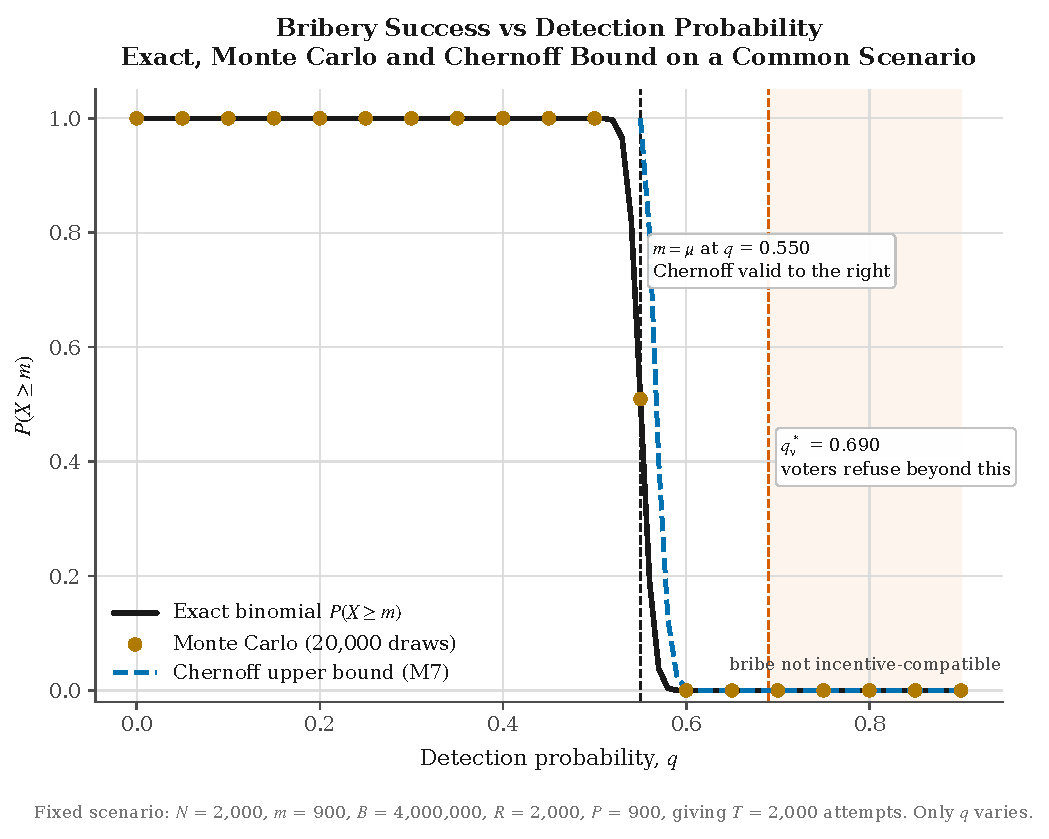
\includegraphics[width=0.86\textwidth]{fig_01_method_comparison.pdf}
\caption[Exact, Monte Carlo and Chernoff comparison]{Exact binomial,
Monte Carlo and Chernoff bound against detection probability on one
fixed scenario. Averaging these three quantities across heterogeneous
randomised trials would compare them on different sub-populations ---
the bound exists only where $m > \mu$ --- so this figure varies only
$q$.}
\label{fig:detection}
\end{figure}

Two mechanisms produce that collapse and they compound. The mean
surviving count $T(1-q)$ falls linearly in $q$, and the binomial
concentrates tightly around its mean, so once the mean crosses the
threshold the tail probability falls away exponentially. On top of
that, bribery carries the rational-voter gate: beyond
$q_v^* = R/(R+P)$ the bribe is refused outright.
\figref{fig:utility} shows that surface, with the closed-form threshold
traced over the numerically computed zero contour. Both are evaluated
by the production modules --- the surface by the M1 implementation, the
curve by the T2 solver --- so their coinciding checks that the solver
returns the root of the utility function as coded. It is a check on the
implementation, not independent evidence for the model: T2 is the
analytic root of M1, so agreement is expected, and only a coding error
could separate the two.

\begin{figure}[H]
\centering
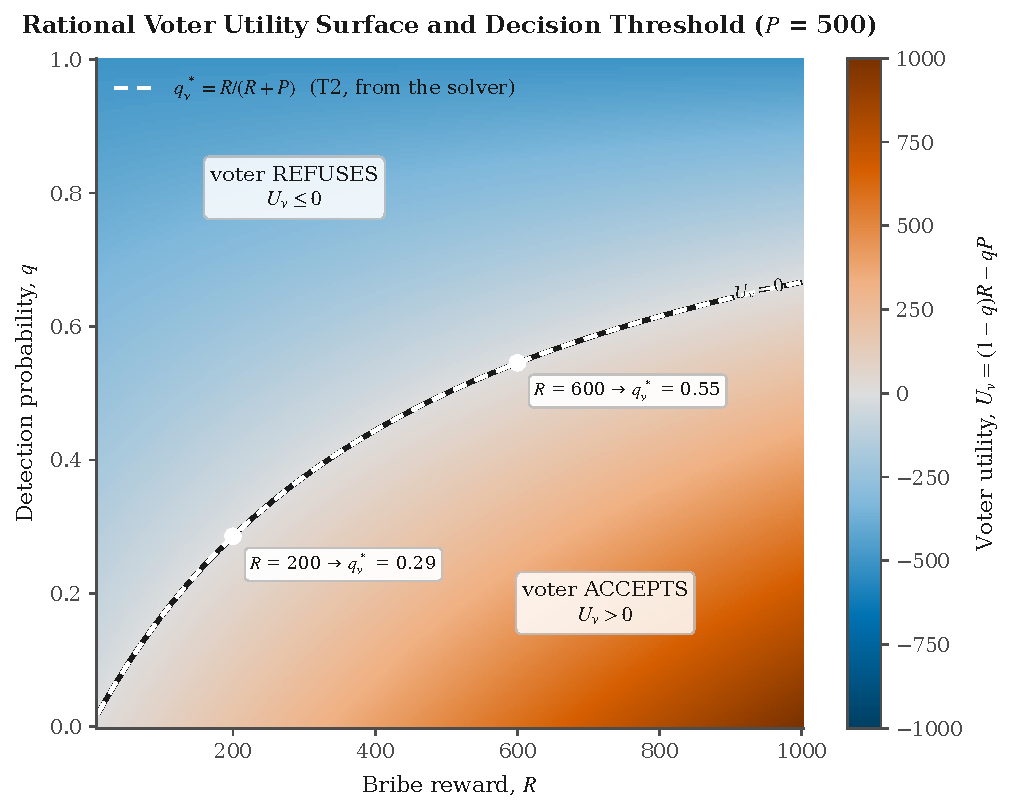
\includegraphics[width=0.78\textwidth]{fig_02_voter_utility_threshold.pdf}
\caption[Voter utility surface and decision threshold]{Rational voter
utility $\Uv = (1-q)R - qP$, with the $\Uv = 0$ decision boundary and
the closed-form indifference threshold $q_v^{*} = R/(R+P)$ drawn
together.}
\label{fig:utility}
\end{figure}

\begin{finding}
\finhead{F1 --- where defensive effort pays (RQ1)}
Budget and detection are not interchangeable. Budget raises success
gradually and saturates at a capacity ceiling that no further spending
moves. Detection produces a sharp collapse, because it lowers the mean
and --- for bribery --- eventually removes the attacker's supply of
willing voters altogether. A defender choosing between raising the cost
of an attack and raising the chance of catching it should prefer the
latter.
\end{finding}

\subsection{F2 --- The three methods agree, and each has a distinct use}
\label{sec:findings-methods}

RQ2 asks how well the Monte Carlo estimate and the Chernoff bound
reproduce the exact value.

The Monte Carlo estimator is accurate: mean absolute error against the
exact binomial probability was \BriberyMCError{} for bribery,
\SybilMCError{} for Sybil and \BallotStuffingMCError{} for ballot
stuffing, with worst-case errors of \BriberyMCMaxError{},
\SybilMCMaxError{} and \BallotStuffingMCMaxError{} respectively.
A convergence sweep over sample sizes from \ConvergenceMinSize{} to
\ConvergenceMaxSize{} draws (\code{results/csv/monte\_carlo\_convergence.csv})
shows the estimator settling to within \ConvergenceTolerance{} of the
exact value from \ConvergenceSettles{} draws onward, reaching an
absolute error of \ConvergenceFinalError{} at the largest sample size.
The \MonteCarloTrials{} draws used per scenario therefore sit inside the
converged regime. A two-standard-error envelope is the looser test here
and is reported in the same file: since it is a 95\% interval, isolated
excursions are expected and two of the nine sample sizes show one, which
is why the settling point is quoted against a fixed tolerance rather
than against the envelope.

The Chernoff bound held in every trial where it was mathematically
defined: \BriberyChernoffHolds\% of \BriberyChernoffValid{} valid
bribery trials, \SybilChernoffHolds\% of \SybilChernoffValid{} Sybil
trials and \BallotStuffingChernoffHolds\% of
\BallotStuffingChernoffValid{} ballot-stuffing trials, with no
violation anywhere. It is also loose --- a mean gap of
\BriberyChernoffGap{} for bribery --- which is the expected behaviour
of a bound rather than a defect.

The bound is one-sided, however, and it exists only where the threshold
sits above the mean. That left the scenarios with $m \leq \mu$ --- the
ones in which the attack is \emph{most} likely to succeed --- with no
analytic statement at all. The two-sided certificate of
Section~\ref{sec:certificate} closes that gap by applying the
$(1-\delta)$ lower-tail form to the failure event, and
\figref{fig:twosided} validates both directions against the exact value
on the same experiment.

\begin{figure}[H]
\centering
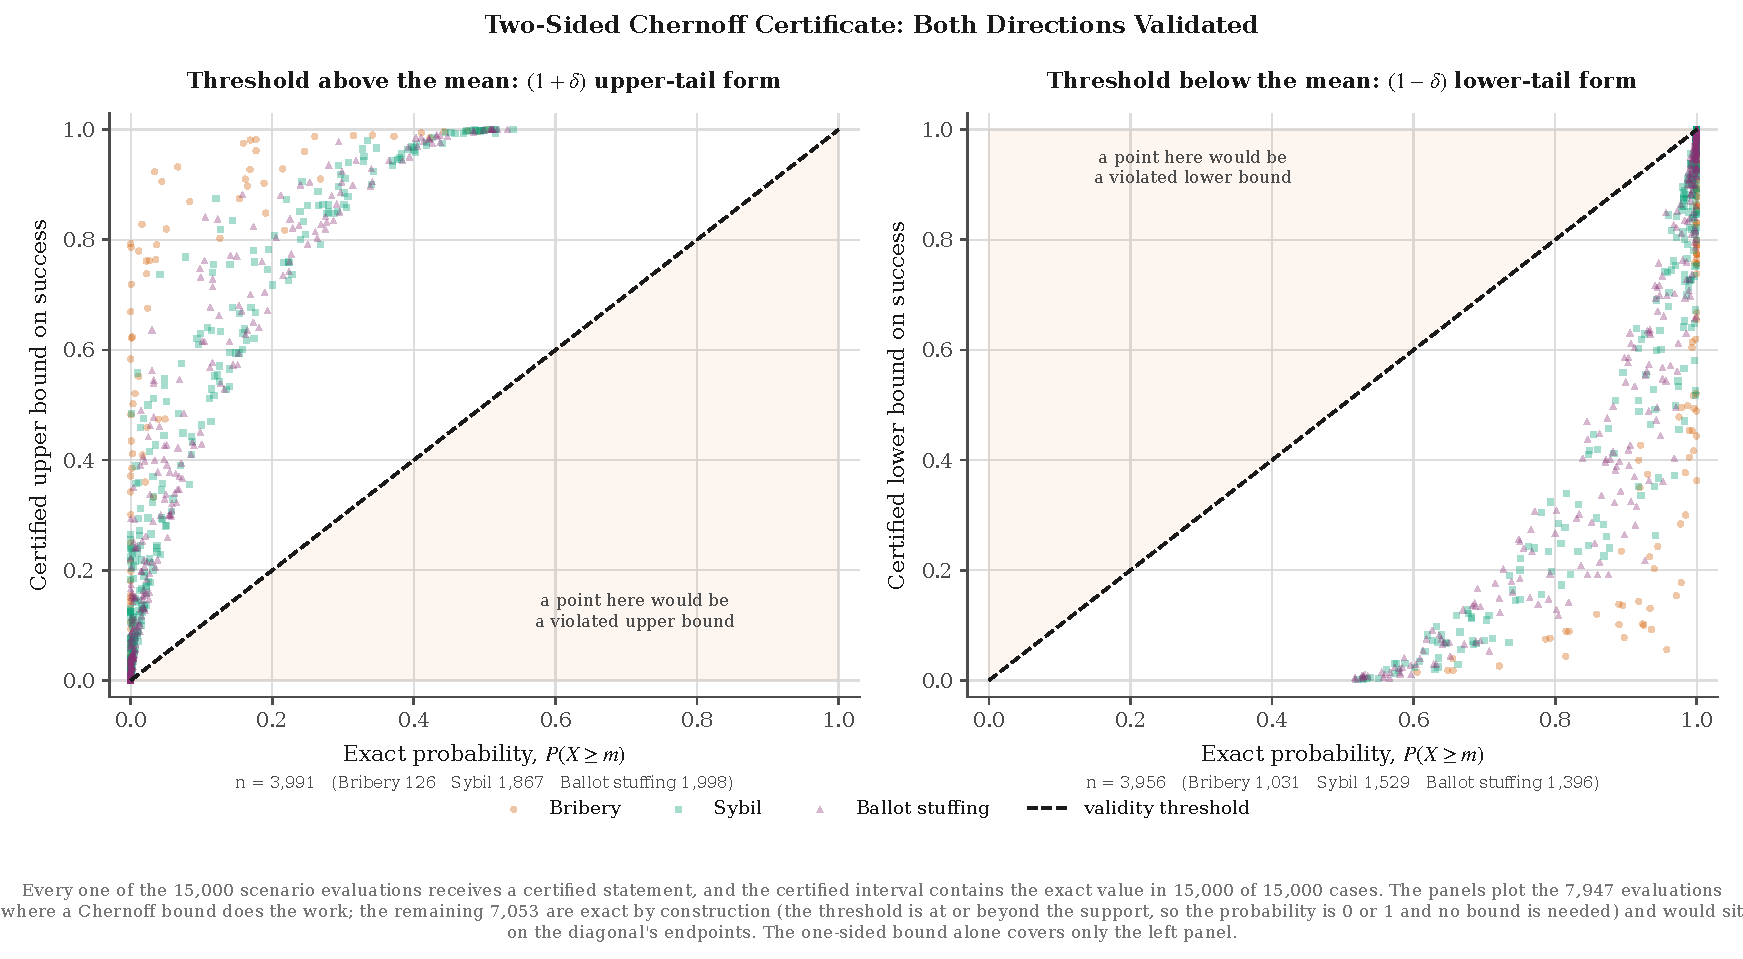
\includegraphics[width=\textwidth]{fig_03_chernoff_two_sided.pdf}
\caption[Two-sided Chernoff certificate]{Both Chernoff directions
validated. Left: threshold above the mean, where the $(1+\delta)$
upper-tail form certifies success from above --- valid points lie on or
above the diagonal. Right: threshold below the mean, where the
$(1-\delta)$ lower-tail form applied to the failure event certifies
success from below --- valid points lie on or below it. No point falls
on the wrong side of either diagonal.}
\label{fig:twosided}
\end{figure}

With the certificate in place, every one of the 15{,}000 scenario
evaluations carries a guaranteed statement, and the certified interval
contains the exact value in 100\% of them.

\begin{finding}
\finhead{F2 --- when to use which method (RQ2)}
Use the exact binomial value whenever it is affordable; it always was
here, even at $N = \SThreeN$. Use Monte Carlo where the quantity has no
closed form --- the concrete election simulation, for instance. Use the
Chernoff bound when a \emph{provable} statement is required rather than
an estimate: it is the only one of the three that certifies a margin as
safe independently of how the simulation ran, which is what makes the
certified margin $m_{\varepsilon}$ meaningful as a security claim
rather than an observation.
\end{finding}

\subsection{F3 --- Countermeasures work, but not uniformly}

Both remaining vectors behave more smoothly than bribery, because
neither has a consent gate: a forged identity does not decline. Their
success probability rises steadily with effort rather than switching
off at a threshold.

Sybil attacks are the most resilient of the three under the tested
parameter distribution, retaining a mean success probability of
\SybilProtected{} under protection --- roughly twice the protected
bribery figure of \BriberyProtected. The reason is structural rather
than numerical: bribery is suppressed twice over, once by detection and
once by the voter's refusal, whereas a Sybil attack is suppressed only
by detection. \figref{fig:comparison} shows the three vectors together.

\begin{figure}[H]
\centering
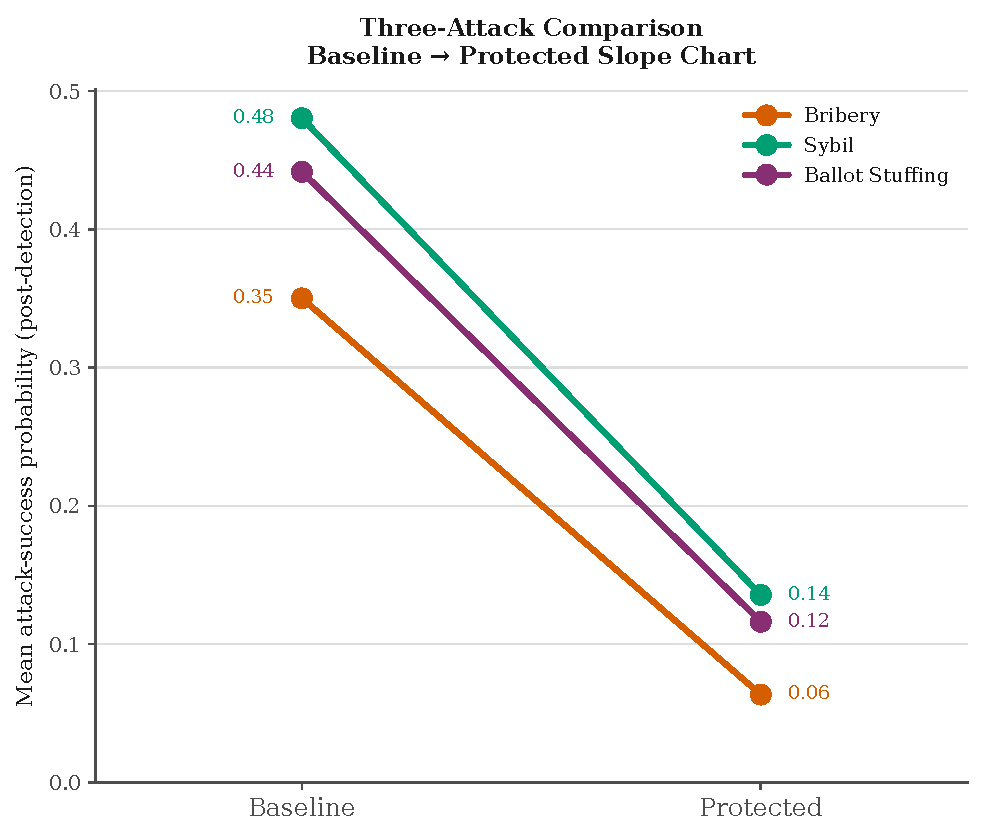
\includegraphics[width=0.64\textwidth]{fig_04_attack_comparison.pdf}
\caption[Three-attack comparison]{Mean success probability for the
three vectors, baseline against protected.}
\label{fig:comparison}
\end{figure}

The distributions add something the means conceal: under protection
they are compressed toward zero rather than merely shifted downward.
The countermeasures remove the upper tail of highly successful attacks,
which is the part of the distribution that actually decides elections.
They do not remove the attack. Under protection the Sybil and
ballot-stuffing vectors retain mean success probabilities of
\SybilProtected{} and \BallotStuffingProtected{} respectively, so the
defensible claim is that attack success is \emph{substantially reduced}
under the modelled countermeasures, not that it is eliminated.

\begin{finding}
\finhead{F3b --- where the residual risk sits}
Identity verification, not vote recording, is the binding constraint.
Sybil attacks remain the most successful vector under protection
(\SybilProtected{} mean success probability) because the ledger's
integrity guarantees say nothing about whether the identity behind a
ballot is real. This is consistent with voter authentication being
repeatedly flagged as an open problem in the systematic
reviews~\cite{ohize2025,rahul2025}. A deployment that hardens the chain
while leaving registration weak has hardened the wrong layer.
\end{finding}

\subsection{F4 --- Chain integrity and election correctness are independent}
\label{sec:findings-concrete}

The results so far are probabilities. \figref{fig:flip} reports what
happened when \ElectionTrials{} elections were genuinely mined on a
proof-of-work chain, attacked, and re-tallied from the chain to see who
actually won.

\begin{figure}[H]
\centering
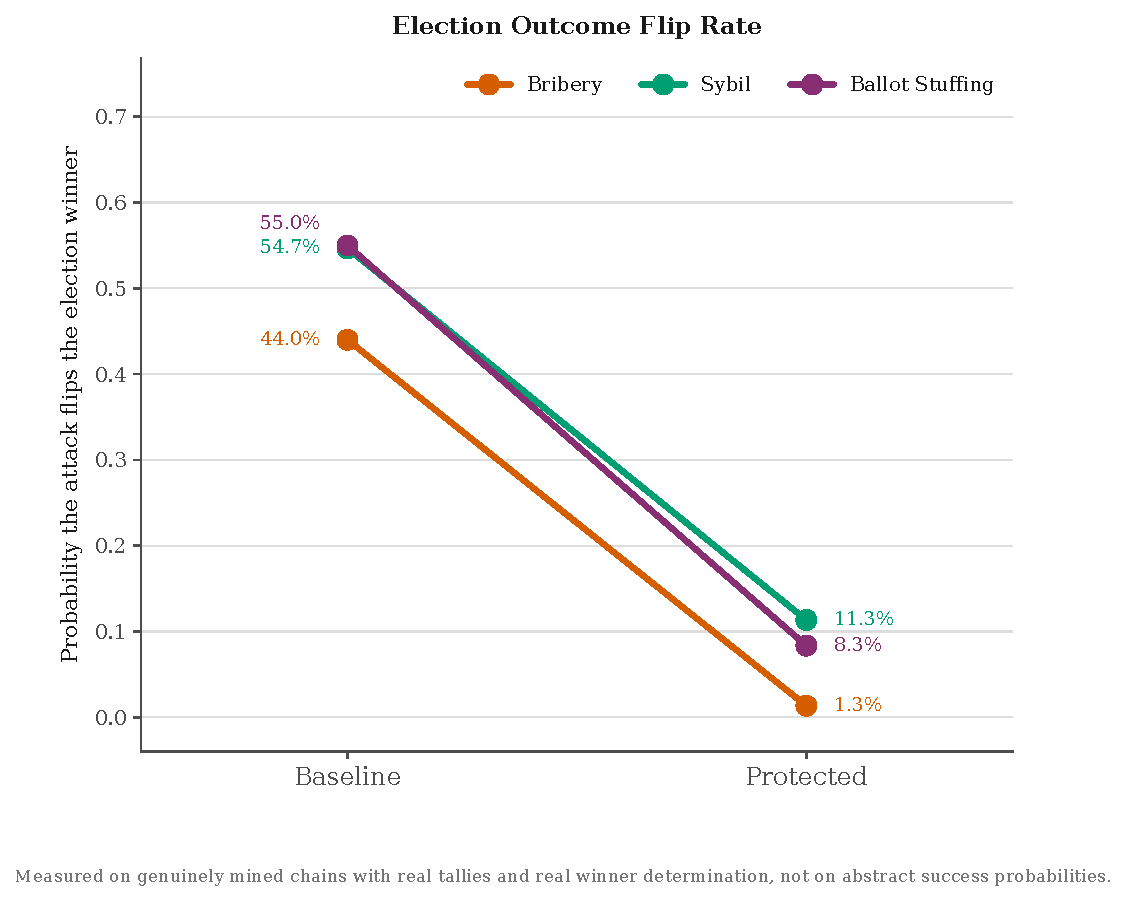
\includegraphics[width=0.64\textwidth]{fig_05_election_flip_rate.pdf}
\caption[Election outcome flip rate]{Probability that an attack flips
the winner of a concrete, blockchain-recorded election.}
\label{fig:flip}
\end{figure}

Baseline flip rates were \FlipBriberyBaseline\% for bribery,
\FlipSybilBaseline\% for Sybil and \FlipBallotStuffingBaseline\% for
ballot stuffing, falling under protection to \FlipBriberyProtected\%,
\FlipSybilProtected\% and \FlipBallotStuffingProtected\%. This is the
cross-layer check that Section~\ref{sec:method-twolayer} exists to
provide: two independent implementations --- one analytic, one a mined
chain --- agree in magnitude, in the direction and size of the
protection effect, and in placing bribery lowest in both layers. They
do not agree on the ordering of the top two: the analytic layer puts
Sybil (\SybilBaseline{}) above ballot stuffing (\BallotStuffingBaseline{}),
while the concrete layer reverses them, at \FlipSybilBaseline\% against
\FlipBallotStuffingBaseline\%. That gap is a third of a percentage point
on \ElectionTrials{} trials per vector --- well inside sampling error ---
so the two vectors are better read as indistinguishable at the concrete
layer than as ranked.

Individual trials make this concrete. For a representative flipped
baseline election, the attacker's surviving fraudulent votes carry the
target past the opponent's tally, while the protected run on the
\emph{same} starting election leaves the original winner in place.

\begin{finding}
\finhead{F4 --- the central observation}
Chain integrity was \ChainIntegrityHeld{} in any of the
\ElectionTrials{} trials. In the \FlipBriberyBaseline\% of baseline
bribery trials that flipped the winner, the blockchain was working
perfectly: every fraudulent vote was correctly formed, correctly mined
and permanently recorded, and the validity check passed afterwards.
Immutability guarantees that a wrong result cannot subsequently be
altered. It does not guarantee that the result is right. This is the
quantitative form of the argument Park et al.~\cite{park2021} make
qualitatively.
\end{finding}

\subsection{F5 --- Deterrence is far cheaper than prevention}
\label{sec:thresholds-results}

\tabref{tab:thresholds} collects every threshold for the five benchmark
scenarios. The critical detection probability $q_d^{*}$ --- the point at
which mounting the attack stops paying --- lies between
\CriticalDetectionMin{} and \CriticalDetectionMax{} across the
\CriticalDetectionBindingCount{} scenarios where detection is the
binding constraint. The protected configuration operates at
$q = \ProtectedQ$, roughly \ProtectionHeadroom{} times higher than the
strongest of those requirements.

\begin{table}[htbp]
\centering
\caption{Critical thresholds for the five benchmark scenarios under the baseline configuration.}
\label{tab:thresholds}
\small
\resizebox{\textwidth}{!}{%
\begin{tabular}{lrrrrrrrrrrr}
\toprule
Scenario & $N$ & $m$ & $R^*$ & $q_v^*$ & $T_{\min}$ & $q_d^*$ & $B^*$ & $T^*$ & $m_\alpha$ & $m_\varepsilon$ & $P(X \geq m)$ \\
\midrule
S1 & 100 & 35 & 52 & 0.118 & 38 & 0.118 & 2,880 & 37 & 34 & --- & 0.423 \\
S2 & 10,000 & 1,943 & 68 & 0.118 & 2,089 & 0.072 & 249,480 & 2,083 & 1,937 & --- & 0.328 \\
S3 & 100,000 & 19,015 & 63 & 0.111 & 20,016 & 0.050 & 2,998,650 & 20,000 & 19,000 & 19,515 & 0.320 \\
S4 & 5,000 & 4,758 & 26 & 0.167 & 5,008 & 0.051 & 499,400 & 5,000 & 4,750 & --- & 0.316 \\
S5 & 5,000 & 550 & 26 & 0.167 & 579 & 0.000 & 57,100 & 0 & 76 & --- & 0.000 \\
\bottomrule
\end{tabular}%
}
\vspace{2pt}
{\footnotesize\textit{Note.} $R^*$ minimum bribe a rational voter accepts (T1); $q_v^*$ voter-indifference detection (T2); $T_{\min}$ attempts for even odds (T3); $q_d^*$ critical detection at which attacking stops paying (T5); $B^*$ break-even budget (T4); $T^*$ utility-maximising attempts; $m_\alpha$ margin beaten at even odds (T7); $m_\varepsilon$ Chernoff-certified safe margin at $\varepsilon = 10^{-3}$ (T6). A dash means the threshold does not exist in the searched domain.}
\end{table}


\begin{figure}[H]
\centering
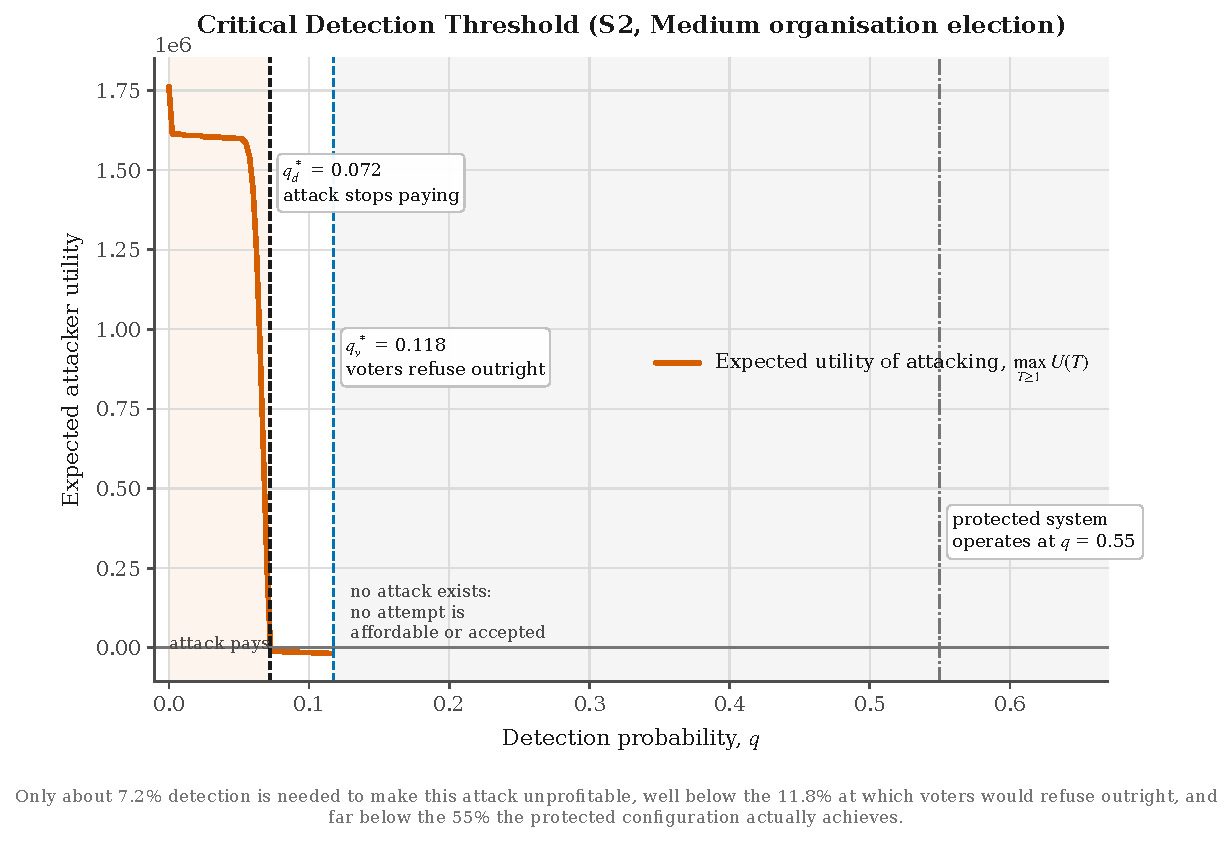
\includegraphics[width=0.80\textwidth]{fig_06_critical_detection.pdf}
\caption[Critical detection threshold]{Expected utility of attacking as
detection rises, for the medium-organisation scenario. Two thresholds
are marked: $q_d^{*}$, where the attack stops paying, and $q_v^{*}$,
where voters refuse outright.}
\label{fig:critical}
\end{figure}

The gap between the two thresholds is worth dwelling on. At $q_d^{*}$
the attack is still perfectly possible --- voters would accept, the
budget suffices --- but a rational attacker declines because the
expected return has gone negative. At $q_v^{*}$ the attack becomes
impossible, because the voters themselves refuse. Deterrence arrives
first and costs less; prevention arrives later and costs more.
\tabref{tab:thresholds} places all five scenarios against both
thresholds; every one of them sits far to the left of the protected
configuration's operating point.

\begin{finding}
\finhead{F5 --- minimum viable defence (RQ4)}
Making bribery unprofitable requires a detection probability of only
\STwoQCritical{} in the medium-organisation scenario and
\SThreeQCritical{} at national scale --- roughly one caught bribe in
fourteen, and one in twenty. This is far below the \ProtectedQ{} the
modelled countermeasures deliver. The security-relevant conclusion is
not that the countermeasures work, but that \emph{much weaker ones
would have}: the expensive part of the defence is buying certainty
rather than deterrence.
\end{finding}

\subsubsection{Break-even budget}

The break-even budget answers the complementary question: how much
would the attacker need before the attempt is worth making?
Sweeping budget for the medium-organisation scenario gives
$B^{*} = \STwoBStar$ against a scenario budget of \STwoBudget. Under the protected configuration the
curve never crosses zero at any budget, because the bribe is not
incentive-compatible at all.

\subsubsection{The contested band of margins}

\tabref{tab:thresholds} gives, for each scenario, the margin the
attacker beats at even odds ($m_\alpha$), the margin actually defended
($m$), and the margin the Chernoff bound certifies as safe
($m_\varepsilon$).

In four of the five scenarios the defended threshold sits inside its
band or a little above the attacker-reachable margin; the exception is
the low-budget scenario S5, where the defended margin exceeds
$m_\alpha$ by a factor of about seven and the attack is out of reach by
a wide margin rather than a narrow one. A certified margin
$m_\varepsilon$ exists for the national-scale scenario only --- in the
others the bound cannot certify even $m = n$ at
$\varepsilon = 10^{-3}$, which the solver reports rather than
silently omitting. At national scale the attacker reaches
\SThreeMReachable{} votes at even odds while the bound certifies safety
only from \SThreeMCertified{} --- a contested band roughly 500 votes
wide, with the defended threshold \SThreeM{} sitting just inside its
lower edge. That is the practical cost of the
bound's conservatism: within that band it declines to certify margins
that are in fact comfortably safe, and only exact computation resolves
them. \figref{fig:pmf} draws the same three thresholds on a single
distribution.

\begin{figure}[H]
\centering
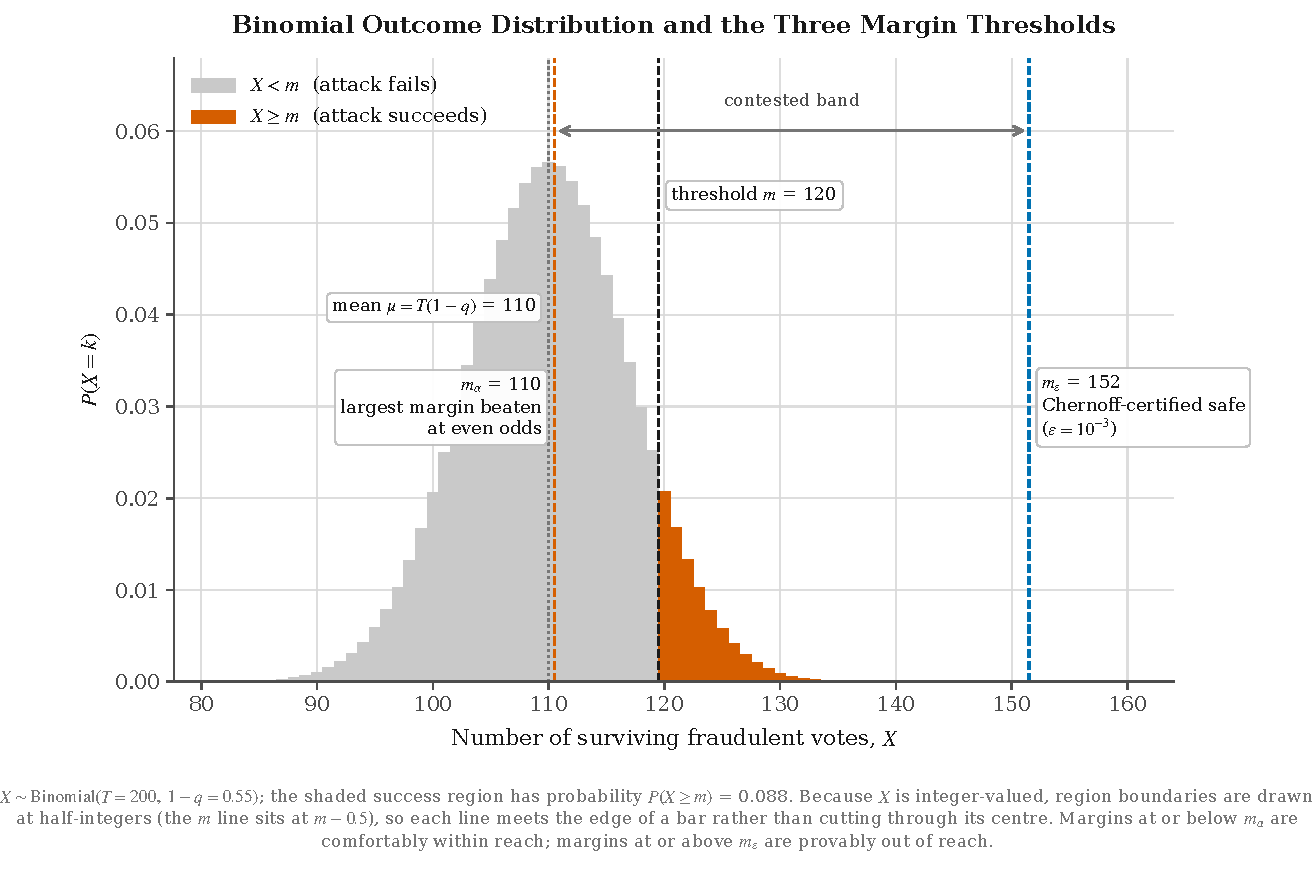
\includegraphics[width=0.86\textwidth]{fig_07_binomial_thresholds.pdf}
\caption[Binomial distribution with margin thresholds]{The binomial
outcome distribution with its mean, the manipulation threshold, the
attacker-reachable margin and the Chernoff-certified safe margin all
marked.}
\label{fig:pmf}
\end{figure}

\subsubsection{The rational attacker does not spend everything}

\figref{fig:optimal} shows expected utility and flip probability
against the number of bribery attempts. Utility is single-peaked: it
rises while further bribes still move the flip probability, then
declines once that probability saturates and each additional bribe buys
only cost and detection risk.

\begin{figure}[H]
\centering
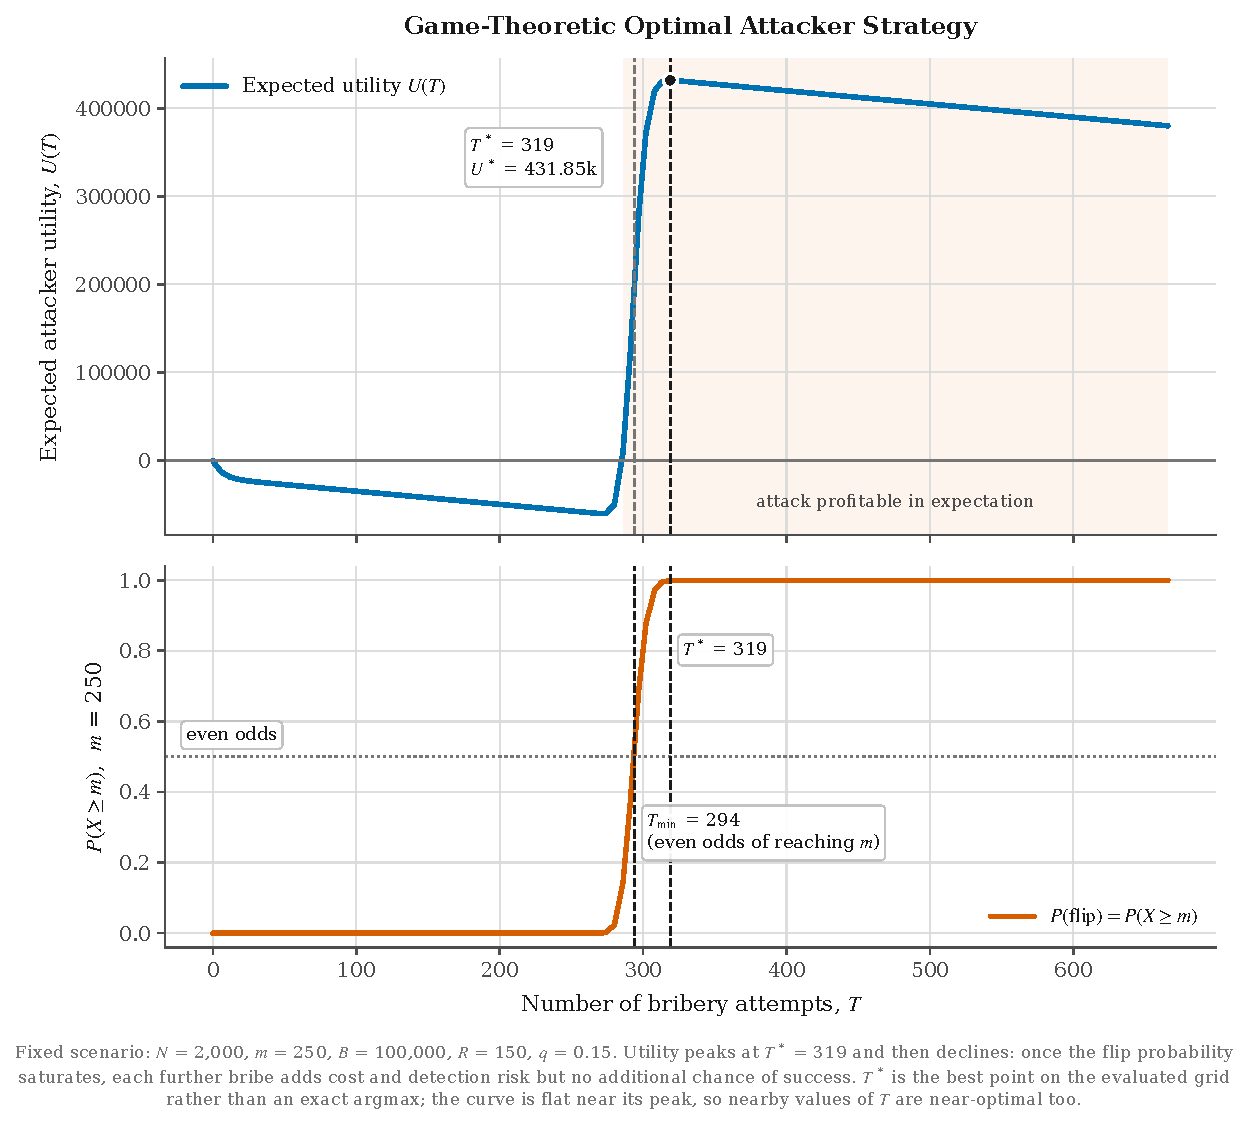
\includegraphics[width=0.80\textwidth]{fig_08_optimal_attacker.pdf}
\caption[Optimal attacker strategy]{Expected attacker utility (top) and
flip probability (bottom) against bribery attempts, with the
utility-maximising $T^{*}$ and the even-odds effort threshold
$T_{\min}$ marked.}
\label{fig:optimal}
\end{figure}

This matters for how the model is read. A budget-exhausting attacker
--- the implicit adversary of many security analyses --- does strictly
worse than a rational one, so optimising a defence against maximum
spending optimises against the wrong opponent. The observation is the
e-voting analogue of the selfish-mining result~\cite{eyal2014}: what an
attacker \emph{would choose} to do, not what they are capable of doing,
is the security-relevant quantity.

\subsection{F6 --- Combining vectors defeats what no single vector can}
\label{sec:coalition}

\subsubsection{No single vector suffices}

Once each vector is held to a realistic capacity ceiling --- forged
registrations limited to \SybilCeilingPct\% of the electorate by the
registration window, injected ballots to \BallotCeilingPct\% by the
turnout anomaly they would otherwise create, in the sense that election
forensics makes detectable~\cite{klimek2012} --- something striking
emerges from \tabref{tab:capacity}. Neither Sybil registration nor
ballot stuffing has an \emph{expected} yield that reaches the
manipulation threshold in any scenario.

The distinction matters and was sharpened after review. The capacity
ratio is $\Ex[X]/m$ --- a mean, not a ceiling. A ratio below one means
the attack falls short \emph{on average}; success is still possible on
an upward fluctuation. What makes the finding hold is how fast that
possibility decays: at S1's bribery ratio of 0.97 the exact success
probability is still \SOneBriberyPFull{}, at S3's ballot-stuffing ratio
of 0.99 it is \SThreeBallotPFull{}, and by a ratio of 0.74 it is
numerically zero. So the accurate statement is that Sybil registration
is effectively out of the running in every scenario, ballot stuffing
retains a small residual chance in the two largest ones, and no single
vector is a reliable route to the threshold --- not that any of them is
arithmetically impossible.

\begin{table}[htbp]
\centering
\caption{Capacity of each vector at full effort, as a multiple of the manipulation threshold $m$ (baseline configuration).}
\label{tab:capacity}
\small
\resizebox{\textwidth}{!}{%
\begin{tabular}{lrrrr}
\toprule
Scenario & Bribery & Sybil & Ballot Stuffing & Combined \\
\midrule
S1 & 0.97 & 0.41 & 0.54 & 1.92 \\
S2 & 1.00 & 0.74 & 0.97 & 2.71 \\
S3 & 1.00 & 0.76 & 0.99 & 2.75 \\
S4 & 1.00 & 0.15 & 0.20 & 1.35 \\
S5 & 0.14 & 0.26 & 0.61 & 1.01 \\
\bottomrule
\end{tabular}%
}
\vspace{2pt}
{\footnotesize\textit{Note.} Values are EXPECTED surviving votes over the threshold, so a value below 1.00 means the mean falls short --- not that the threshold is unreachable. Success remains possible on an upward fluctuation, though its probability collapses quickly: at a ratio of 0.97 the exact $P(X \geq m)$ is still 0.42 for bribery in S1, while by a ratio of 0.74 it is numerically zero. Every entry here falls below 1.00; the budget-feasible optimal coalition clears it in four of the five scenarios (\tabref{tab:coalition}).}
\end{table}


\begin{figure}[H]
\centering
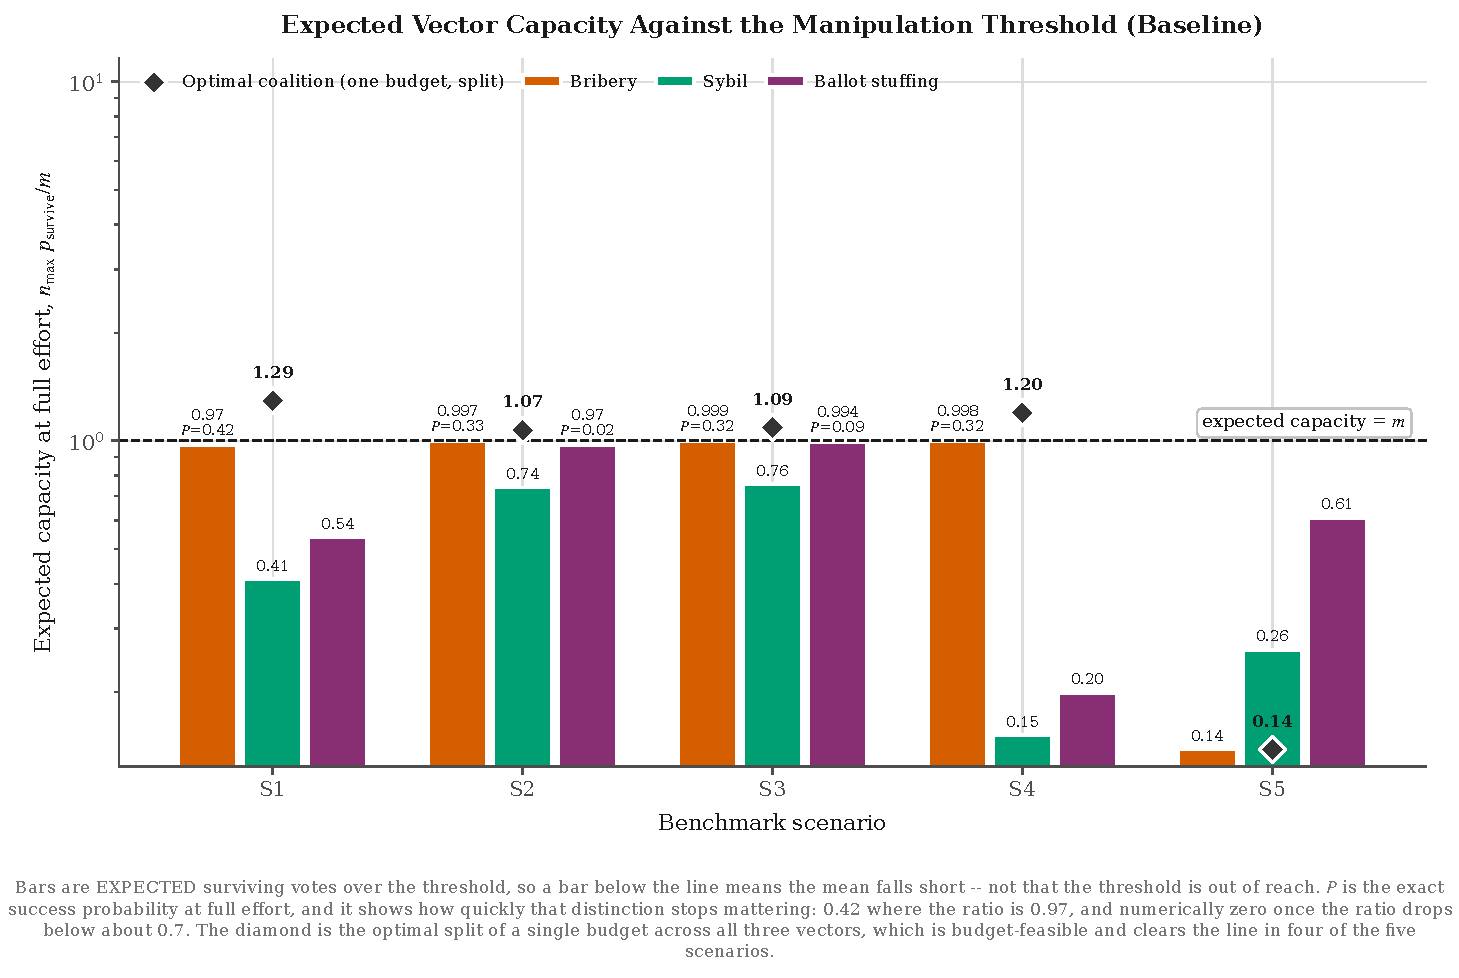
\includegraphics[width=0.86\textwidth]{fig_09_vector_capacity.pdf}
\caption[Vector capacity against the threshold]{\emph{Expected}
capacity of each vector at full effort, as a multiple of the
manipulation threshold. A bar below the line means the mean falls
short, not that the threshold is unreachable --- the annotated $P$ is
the exact success probability at full effort. The diamond is the
optimal split of a single budget across all three vectors, which is
budget-feasible.}
\label{fig:capacity}
\end{figure}

Analysed one vector at a time, this reads as a reassuring result: no
single vector is a dependable route to the threshold, and two of the
three are hopeless. It is the wrong conclusion, and the reason it is
wrong is that the attacker is not obliged to choose.

\subsubsection{The mixed strategy}
\label{sec:findings-coalition}

The search evaluates every way of splitting a single budget across the
three vectors, at a 0.05 resolution over the budget simplex, whose
corners are exactly the pure single-vector strategies. The optimum
leaves the corners in four of the five scenarios: it is strictly
interior in S1 $(0.35, 0.25, 0.40)$ and sits on an edge --- two vectors
funded, one not --- in S2, S3 and S4. Only S5, where no allocation
succeeds at all, returns a corner. The gain therefore comes from mixing
\emph{at least} two vectors rather than from using all three.

\begin{table}[htbp]
\centering
\caption{Optimal multi-vector budget allocation per scenario (baseline configuration).}
\label{tab:coalition}
\small
\resizebox{\textwidth}{!}{%
\begin{tabular}{lrrrrrlrr}
\toprule
Scenario & Bribery & Sybil & Ballot & $\mu_{\mathrm{total}}$ & Coalition $P$ & Best pure & Pure $P$ & Gain \\
\midrule
S1 & 35\% & 25\% & 40\% & 45 & 0.999 & Bribery & 0.423 & 0.576 \\
S2 & 0\% & 5\% & 95\% & 2,077 & 1.000 & Bribery & 0.328 & 0.672 \\
S3 & 0\% & 5\% & 95\% & 20,700 & 1.000 & Bribery & 0.320 & 0.680 \\
S4 & 10\% & 0\% & 90\% & 5,695 & 1.000 & Bribery & 0.316 & 0.684 \\
S5 & 100\% & 0\% & 0\% & 76 & 0.000 & Bribery & 0.000 & 0.000 \\
\bottomrule
\end{tabular}%
}
\vspace{2pt}
{\footnotesize\textit{Note.} Shares are the fractions of one budget allocated to each vector. Coalition success probability is computed exactly, by convolving the three binomial distributions rather than approximating their sum.}
\end{table}


\begin{figure}[H]
\centering
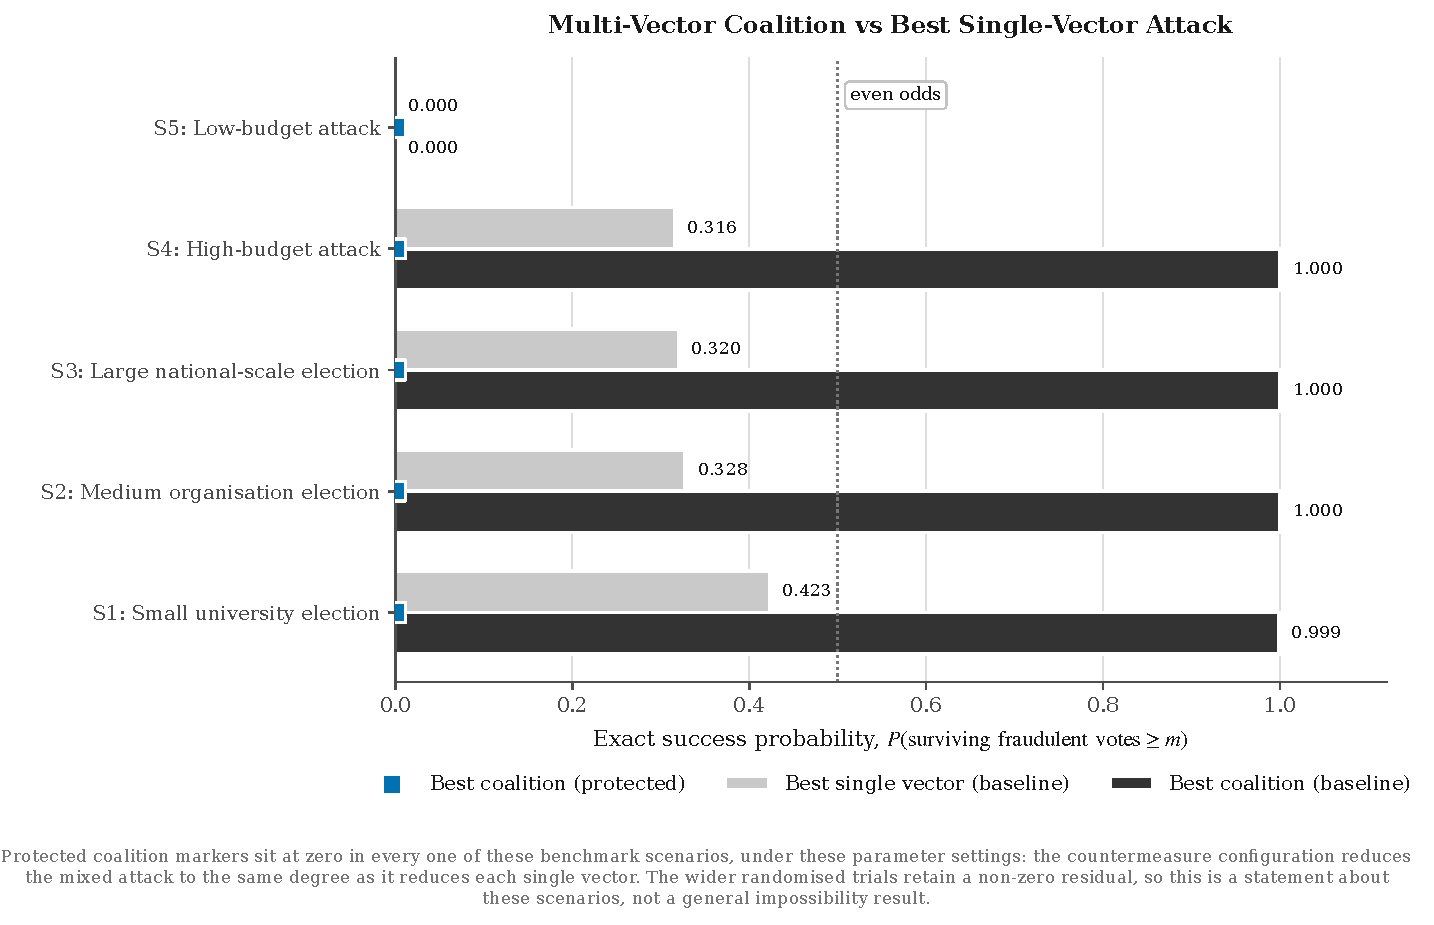
\includegraphics[width=0.88\textwidth]{fig_10_coalition_vs_pure.pdf}
\caption[Coalition against best single vector]{Best coalition attack
against best single-vector attack per scenario, with protected
coalition results overlaid.}
\label{fig:coalition}
\end{figure}

\begin{finding}
\finhead{F6 --- multi-vector attacks (RQ5)}
The optimal mixed strategy strictly outperforms the best single-vector
strategy in \CoalitionBetterCount{} of \CoalitionScenarioCount{}
baseline scenarios, raising mean success probability from
\BestPureMeanBaseline{} to \CoalitionMeanBaseline{}. In the high-budget
scenario, no single vector exceeds a success probability of
\SFourExactFlip{}, yet the mixture reaches near-certainty. A security
evaluation conducted one vector at a time therefore understates the
achievable attack --- not marginally, but qualitatively, by declaring
infeasible an attack that succeeds.
\end{finding}

The mechanism is capacity, not probability. Each vector saturates its
own ceiling long before the budget is exhausted, leaving money that
buys nothing more in that vector but a great deal in another.
Diversification here is not about hedging risk; it is about escaping a
binding constraint.

\subsubsection{Robustness of the coalition finding}

The coalition result depends on assumed relative costs and capacity
ceilings, none of which is empirically grounded.
The analysis therefore re-runs across \SensitivityConfigs{}
combinations of all four constants.

The coalition was at least as good as the best pure strategy in
\SensitivityAtLeastAsGood\% of configurations and strictly better in
\SensitivityStrictlyBetter\%. The qualitative conclusion does not
depend on the particular costs assumed --- as it should not, since a
mixed strategy can never be worse than the best pure one, the pure
strategies being corners of the same simplex. What the sweep
establishes is that the \emph{strict} improvement is not an artefact of
one convenient parameterisation.

\subsubsection{Countermeasures against the coalition}

Across the \CoalitionScenarioCount{} benchmark scenarios, the protected
configuration suppresses the coalition attack to the same degree as it
suppresses each vector alone: mean coalition success probability under
protection is \CoalitionMeanProtected{}. That figure is exactly zero
for these particular benchmark scenarios under these parameter
settings, and should be read as such rather than as a general claim
that the mixed attack is impossible --- the randomised trials, which
sample far more widely, leave a residual success probability of
\SybilProtected{} for Sybil attacks and \BallotStuffingProtected{} for
ballot stuffing. The bribery
gate closes in all \CoalitionScenarioCount{} scenarios, since
$\ProtectedQ > q_v^{*}$ everywhere, and the tightened acceptance and
detection probabilities pull the other two vectors' capacity below the
threshold. Coalition attacks are more dangerous than the single-vector
analysis suggests, but they are not differently defended.

\subsection{Scale effects}

One further result bears on deployment, and it is not uniform across
the vectors. Holding the manipulation threshold at a fixed 10\% of the
electorate and growing $N$, bribery success collapses from
\ScaleBriberySmall{} to \ScaleBriberyLarge{} and ballot stuffing from
\ScaleBallotSmall{} to \ScaleBallotLarge{}, because the attacker's
budget ceiling $T = \lfloor B/R \rfloor$ does not scale with $N$ while
the threshold does.

Sybil registration behaves in the opposite direction, rising from
\ScaleSybilSmall{} to \ScaleSybilLarge{}, and the reason is structural:
its attempt count is a fixed \emph{fraction} of the electorate ---
forged registrations are capped at \SybilCeilingPct\% of $N$ --- so
unlike a fixed budget it scales with the threshold it has to beat, and
the binomial concentrates around a mean that stays a constant multiple
of $m$. The budget argument simply does not apply to a vector whose
capacity is denominated in voters rather than in currency. This is the
scale-effect result stated precisely: growth protects against
\emph{budget-bound} vectors, not against \emph{proportionally
capped} ones.

The implication is not that large elections are safe. It is that large
elections are safe \emph{against a fixed budget}, and that the relevant
attacker for a national election is correspondingly better resourced
--- which is exactly what scenario S3 models, with a budget of
\SThreeBudget{} and a resulting baseline flip probability of
\SThreeExactFlip.


\section{Discussion}

\subsection{What the ledger does and does not buy}

The clearest result in this dissertation is also the least flattering to the technology
it evaluates. Chain integrity held in every one of the \ElectionTrials{} concrete
elections, and in \FlipBriberyBaseline\% of baseline bribery trials the attacker still
changed the winner. Immutability and correctness are orthogonal properties. A ledger
guarantees that what was recorded stays recorded; whether it should have been recorded
is decided upstream, by identity verification, ballot validation and the incentives
facing voters.

This is not an argument against blockchain voting so much as an argument about where
its security budget belongs. The largest measured residual risk under protection is Sybil
registration (\SybilProtected{} mean success probability, roughly twice the protected
bribery figure), which is exactly the vector the ledger does nothing about. Ballot
stuffing is close behind at \BallotStuffingProtected{}, so the residual is better
described as concentrated in the two vectors that bypass the voter rather than in
identity verification alone.

\subsection{Deterrence is cheaper than prevention}

The threshold analysis produces the most actionable finding. Making an attack
unprofitable requires between four and eleven times less detection capability than the
modelled countermeasures deliver: detection probabilities of \CriticalDetectionMin{} to
\CriticalDetectionMax{} suffice across the \CriticalDetectionBindingCount{} scenarios
where detection is the binding constraint, against \ProtectedQ{} provided. In the fifth
scenario the attack is unprofitable at every detection level, so no threshold exists. If detection is expensive and
roughly linear in cost --- a reasonable assumption for audit sampling and identity
checks --- then most of the spend is buying certainty rather than deterrence.

Two caveats keep this from being a licence to under-invest. Deterrence assumes a
rational attacker who computes expected utility and declines when it is negative; an
attacker with non-monetary motives, or one who misjudges the detection rate, is not
deterred by an unfavourable expectation. And $q_d^{*}$ depends on the payoff $V$ and
penalty $D$, which are the least well-grounded parameters in the model. The
qualitative conclusion --- deterrence thresholds sit well below prevention thresholds
--- is robust; the specific numbers should be read as illustrative.

\subsection{Single-vector analysis is not conservative}

It is tempting to treat a per-vector evaluation as conservative, on the reasoning that
each attack is assessed at full strength. The coalition results show this is backwards.
Two of the three vectors have an expected yield below the threshold in every scenario,
and combining them produced near-certain success in four of five. Single-vector analysis
did find an attack: bribery was viable in \BestPureViableCount{} of the
\CoalitionScenarioCount{} scenarios, with success probabilities from \BestPureMin{} to
\BestPureMax{}. But it is the difference between a roughly one-in-three chance and a
near-certainty that matters to a defender, and only the coalition analysis surfaces the
latter.

The generalisable point is that capacity ceilings, not success probabilities, are what
compose badly. Each ceiling is a hard limit within its own vector and irrelevant across
vectors, so an attacker who spreads effort escapes all three at once. Any security
argument resting on ``the attacker cannot obtain enough of X'' should be checked against
an attacker who does not need all of it from X.

\subsection{Answers to the research questions}

\begin{description}[leftmargin=1.2em,style=nextline,itemsep=4pt]
\item[RQ1] Success probability rises with budget and falls with detection, but the two
  are not symmetric. Budget effects are gradual and saturate at the capacity ceiling;
  detection effects are sharp, with success collapsing over a narrow band of $q$ once
  the mean falls below the threshold. Detection is the more efficient lever.
\item[RQ2] Monte Carlo reproduced the exact probability to a mean absolute error of
  \BriberyMCError{} for bribery (\SybilMCError{} and \BallotStuffingMCError{} for the
  other two) and is the right tool where no closed form exists. The Chernoff bound never
  failed but was loose, by a mean of \BriberyChernoffGap{} for bribery and
  \SybilChernoffGap{} and \BallotStuffingChernoffGap{} for the others; its value is that
  it \emph{proves} rather than estimates.
\item[RQ3] The protected configuration reduced success probability by
  \BriberyRelReduction\%, \SybilRelReduction\% and \BallotStuffingRelReduction\% for the
  three vectors, and real winner-flip rates by up to \FlipBriberyRelReduction\%.
  The two largest residuals are Sybil (\SybilProtected{}) and ballot stuffing
  (\BallotStuffingProtected{}), both above the protected bribery figure of
  \BriberyProtected{}; the largest is Sybil, the vector the ledger does nothing about.
\item[RQ4] Critical detection thresholds lie between \CriticalDetectionMin{} and
  \CriticalDetectionMax{} in the \CriticalDetectionBindingCount{} of
  \CoalitionScenarioCount{} scenarios where detection is the binding constraint --- far
  below what the modelled countermeasures deliver. In the remaining scenario the attack
  never pays at any detection level.
\item[RQ5] Yes. Mixed strategies strictly beat the best single vector in
  \CoalitionBetterCount{} of \CoalitionScenarioCount{} scenarios, and the effect survives
  a \SensitivityConfigs-configuration robustness sweep.
\end{description}

%=======================================================================
\section{Limitations and threats to validity}
\label{sec:limitations}

\textbf{Independence.} Attempts are modelled as independent Bernoulli trials with
constant per-scenario probabilities. Real manipulation is correlated: a briber who finds
one willing voter in a community finds more, and a detection mechanism that catches one
forged registration often catches the batch. Positive correlation increases the variance
of the outcome count without changing its mean, which fattens both tails --- so the
model likely understates both the best and worst cases. The direction of the effect on
$\Prob(X \geq m)$ depends on which side of the mean the threshold sits, which is
precisely the contested-band question of Section~\ref{sec:thresholds-results}.

\textbf{Homogeneous voters.} All voters facing the same $(q, R, P)$ reach the same
decision, so the acceptance gate is binary at the population level. Real electorates are
heterogeneous, and a distribution over reservation prices would replace the sharp gate
with a smooth response curve. This is the single most consequential simplification in
the bribery model and the most obvious extension.

\textbf{Parameter grounding.} The probabilities, the payoff $V$, the penalty $D$ and the
relative costs of the three vectors are plausible but not empirically calibrated. No
public dataset gives the probability that a forged voter registration is detected. The
sensitivity sweep addresses this for the coalition result; the threshold values should
be read as illustrative of magnitude, not as measurements.

\textbf{The blockchain is educational.} The implementation mines real proof-of-work
blocks and detects real tampering, but it is a single-process chain. It has no peer-to-peer
network, no fork resolution, no economic security and no adversarial nodes.
Consensus-layer attacks are consequently out of scope entirely.

\textbf{Countermeasures as probabilities.} Modelling identity verification as
``catches a forgery with probability $p_d$'' says nothing about how to achieve any
particular $p_d$, and real mechanisms fail in correlated, adversarially-chosen ways
rather than independently at a fixed rate.

\textbf{Scope.} Coercion, receipt-freeness, client-side malware, denial of service and
consensus attacks are all excluded. A coerced voter differs from a bribed one in a way
this model cannot express: the utility calculation of \eqnref{eq:m1} assumes the voter
may decline.

%=======================================================================
\section{Conclusion and future work}

This dissertation modelled three e-voting manipulation vectors probabilistically and
game-theoretically, evaluated them over \TotalTrials{} matched randomised trials and
\ElectionTrials{} genuinely mined elections, and inverted the model to find the
parameter values at which each attack ceases to be viable.

The measured effect of the protected configuration is substantial --- relative
reductions of \BriberyRelReduction\%, \SybilRelReduction\% and
\BallotStuffingRelReduction\% in success probability, and up to
\FlipBriberyRelReduction\% in real winner-flip rate. But the two findings that seem most
worth carrying forward are the ones the aggregate numbers obscure. Attacks stop being
worth mounting at detection probabilities between \CriticalDetectionMin{} and
\CriticalDetectionMax{} in the \CriticalDetectionBindingCount{} scenarios where detection
binds --- between four and eleven times below what a fully protected system provides ---
so deterrence is much cheaper than prevention. And an attacker who splits one budget
across all three vectors beats the best single-vector attacker in
\CoalitionBetterCount{} of \CoalitionScenarioCount{} scenarios, turning a roughly
one-in-three chance into a near-certainty --- so evaluating vectors independently is not
the conservative choice it appears to be.

Underneath both sits the observation that motivated the work. Chain integrity was
\ChainIntegrityHeld{} in any trial, and elections were stolen anyway. The ledger
faithfully recorded fraudulent votes as fraudulent votes, permanently and verifiably.
Whatever blockchain-based voting is for, it is not for this.

\subsection*{Future work}

Four extensions follow directly. Replacing the homogeneous voter with a distribution
over reservation prices would turn the acceptance gate into a response curve and is the
most natural next step. Introducing correlation between attempts, via a beta-binomial or
an explicit contagion model, would test the independence assumption that the current
tails depend on. Extending the coalition framework to a defender who allocates a
detection budget across vectors would turn the analysis into a two-player game with a
computable equilibrium, of which the present work computes only the attacker's best
response. Finally, calibrating any of the probabilities against real electoral-fraud
audit data would convert the illustrative threshold values into a usable defensive
specification.

%=======================================================================
\clearpage
\addcontentsline{toc}{section}{References}
\begin{thebibliography}{99}

\bibitem{adida2008} B.~Adida. Helios: Web-based Open-Audit Voting. In
\emph{Proceedings of the 17th USENIX Security Symposium}, pp.~335--348, 2008.

\bibitem{becker1968} G.~S.~Becker. Crime and Punishment: An Economic Approach.
\emph{Journal of Political Economy}, 76(2):169--217, 1968.

\bibitem{benaloh1994} J.~Benaloh and D.~Tuinstra. Receipt-Free Secret-Ballot
Elections (Extended Abstract). In \emph{Proceedings of the 26th Annual ACM
Symposium on Theory of Computing (STOC)}, pp.~544--553, 1994.

\bibitem{borge2017} M.~Borge, E.~Kokoris-Kogias, P.~Jovanovic, L.~Gasser,
N.~Gailly and B.~Ford. Proof-of-Personhood: Redemocratizing Permissionless
Cryptocurrencies. In \emph{IEEE European Symposium on Security and Privacy
Workshops (EuroS\&PW)}, pp.~23--26, 2017.

\bibitem{chernoff1952} H.~Chernoff. A Measure of Asymptotic Efficiency for Tests
of a Hypothesis Based on the Sum of Observations. \emph{Annals of Mathematical
Statistics}, 23(4):493--507, 1952.

\bibitem{daian2018} P.~Daian, T.~Kell, I.~Bentov and A.~Juels. On-Chain Vote
Buying and the Rise of Dark DAOs. \emph{Hacking, Distributed} (IC3 technical
report), July 2018. Available at
\url{https://hackingdistributed.com/2018/07/02/on-chain-vote-buying/}.
\emph{Cited as a technical report; not peer reviewed.}

\bibitem{douceur2002} J.~R.~Douceur. The Sybil Attack. In \emph{Proceedings of
the 1st International Workshop on Peer-to-Peer Systems (IPTPS)}, LNCS 2429,
pp.~251--260, 2002.

\bibitem{eyal2014} I.~Eyal and E.~G.~Sirer. Majority Is Not Enough: Bitcoin
Mining Is Vulnerable. In \emph{Financial Cryptography and Data Security (FC)},
LNCS 8437, pp.~436--454, 2014.

\bibitem{faliszewski2009} P.~Faliszewski, E.~Hemaspaandra and
L.~A.~Hemaspaandra. How Hard Is Bribery in Elections? \emph{Journal of
Artificial Intelligence Research}, 35:485--532, 2009.

\bibitem{juels2005} A.~Juels, D.~Catalano and M.~Jakobsson. Coercion-Resistant
Electronic Elections. In \emph{Proceedings of the 2005 ACM Workshop on Privacy
in the Electronic Society (WPES)}, pp.~61--70, 2005.

\bibitem{klimek2012} P.~Klimek, Y.~Yegorov, R.~Hanel and S.~Thurner.
Statistical Detection of Systematic Election Irregularities. \emph{Proceedings
of the National Academy of Sciences}, 109(41):16469--16473, 2012.

\bibitem{liu2019} Z.~Liu, N.~C.~Luong, W.~Wang, D.~Niyato, P.~Wang,
Y.-C.~Liang and D.~I.~Kim. A Survey on Applications of Game Theory in
Blockchain. \emph{arXiv preprint} arXiv:1902.10865, 2019.

\bibitem{mccorry2017} P.~McCorry, S.~F.~Shahandashti and F.~Hao. A Smart
Contract for Boardroom Voting with Maximum Voter Privacy. In \emph{Financial
Cryptography and Data Security (FC)}, LNCS 10322, pp.~357--375, 2017.

\bibitem{mitzenmacher2017} M.~Mitzenmacher and E.~Upfal. \emph{Probability and
Computing: Randomization and Probabilistic Techniques in Algorithms and Data
Analysis}. 2nd ed., Cambridge University Press, 2017.

\bibitem{nakamoto2008} S.~Nakamoto. \emph{Bitcoin: A Peer-to-Peer Electronic
Cash System}. 2008.

\bibitem{ohize2025} H.~O.~Ohize, A.~J.~Onumanyi, B.~U.~Umar, L.~A.~Ajao,
R.~O.~Isah, E.~M.~Dogo, B.~K.~Nuhu, O.~M.~Olaniyi, J.~G.~Ambafi, V.~B.~Sheidu
and M.~M.~Ibrahim. Blockchain for Securing Electronic Voting Systems: A Survey
of Architectures, Trends, Solutions, and Challenges. \emph{Cluster Computing},
28, 2025. DOI 10.1007/s10586-024-04709-8.

\bibitem{park2021} S.~Park, M.~Specter, N.~Narula and R.~L.~Rivest. Going from
Bad to Worse: From Internet Voting to Blockchain Voting. \emph{Journal of
Cybersecurity}, 7(1):tyaa025, 2021.

\bibitem{rahul2025} Rahul, P.~Gulia and N.~S.~Gill. Articulation of Blockchain
Enabled E-Voting Systems: A Systematic Literature Review. \emph{Peer-to-Peer
Networking and Applications}, 18:142, 2025. DOI 10.1007/s12083-025-01956-3.

\bibitem{specter2020} M.~A.~Specter, J.~Koppel and D.~Weitzner. The Ballot is
Busted Before the Blockchain: A Security Analysis of Voatz, the First Internet
Voting Application Used in U.S. Federal Elections. In \emph{Proceedings of the
29th USENIX Security Symposium}, pp.~1535--1553, 2020.

\bibitem{springall2014} D.~Springall, T.~Finkenauer, Z.~Durumeric, J.~Kitcat,
H.~Hursti, M.~MacAlpine and J.~A.~Halderman. Security Analysis of the Estonian
Internet Voting System. In \emph{Proceedings of the 2014 ACM SIGSAC Conference
on Computer and Communications Security (CCS)}, pp.~703--715, 2014.

\end{thebibliography}

%=======================================================================
\clearpage
\appendix
\section{Figure catalogue}

The dissertation uses \FigureCount{} figures. The set is deliberately
small: an earlier draft generated thirty, of which several were
variations on a single point, and the important figures were diluted by
the rest. Each of the ten below carries a distinct step of the argument,
and none can be removed without losing a claim the dissertation makes.

Figure numbers match the generated filenames --- \code{fig\_07\_*} is
Figure 7 --- and \code{check\_consistency.py} fails the build if the two
ever drift apart. Every figure is produced by \code{generate\_figures.py}
from the experimental output at 320\,DPI raster and vector PDF, and
carries a machine-generated caption in
\code{results/FIGURE\_CAPTIONS.md}; none is drawn by hand.

\begin{center}
\small
\begin{tabular}{@{}rp{6.3cm}p{5.6cm}@{}}
\toprule
\textbf{Fig.} & \textbf{Subject} & \textbf{Carries} \\
\midrule
1  & Method comparison: exact, Monte Carlo and Chernoff against detection probability
   & Cross-validation of the three methods; the detection collapse (RQ1, RQ2) \\
\addlinespace
2  & Rational voter utility surface and decision threshold
   & The consent gate that stops bribery independently of detection \\
\addlinespace
3  & Two-sided Chernoff certificate, both directions validated
   & That every scenario carries a proved guarantee (RQ2) \\
\addlinespace
4  & Three-attack comparison, baseline against protected
   & The headline countermeasure effect, and where residual risk sits (RQ3) \\
\addlinespace
5  & Election outcome flip rate on mined chains
   & That integrity and correctness are independent properties \\
\addlinespace
6  & Critical detection threshold $q_d^{*}$
   & How much detection is actually required (RQ4) \\
\addlinespace
7  & Binomial distribution with the three margin thresholds
   & What ``attack success'' means, and the contested band \\
\addlinespace
8  & Game-theoretic optimal attacker strategy
   & That a rational attacker stops short of spending everything (RQ1) \\
\addlinespace
9  & Vector capacity against the manipulation threshold
   & Why no single vector suffices on its own \\
\addlinespace
10 & Coalition against best single-vector attack
   & That mixing vectors beats committing to one (RQ5) \\
\bottomrule
\end{tabular}
\end{center}

The analyses that earlier drafts illustrated with additional figures ---
the budget sweep, the feasibility surface, the electorate-size sweep, the
break-even budget, the contested-margin band, the coalition simplex and
the cost-sensitivity sweep --- all still run, and their outputs remain in
\code{results/csv/}. Only the figures were removed; no result was.

\section{Reproducing these results}

\begin{enumerate}[leftmargin=1.8em,itemsep=2pt]
\item \code{pip install -r requirements.txt}
\item \code{python run\_experiments.py --trials \TotalTrials{} --seed \Seed} \hfill
      randomised paired trials
\item \code{python run\_election\_attacks.py --trials \ElectionTrials{} --seed \Seed}
      \hfill concrete mined elections
\item \code{python run\_threshold\_analysis.py} \hfill thresholds and coalition
\item \code{python generate\_figures.py} \hfill all \FigureCount{} figures and captions
\item \code{python generate\_tables.py} \hfill CSV and \LaTeX{} tables
\item \code{python generate\_report.py} \hfill the dissertation
\item \code{python build\_compendium.py} \hfill the figures-and-results compendium
\item \code{python build\_submission.py} \hfill this document (dissertation + appendix)
\item \code{python check\_consistency.py} \hfill text-versus-data drift check
\item \code{pytest -q} \hfill \TestCount{} tests
\end{enumerate}

Every \emph{experimental result} printed in this report is injected at build time from
\code{results/json/} and \code{results/csv/} by \code{generate\_report.py} rather than
typed. The exceptions are deliberate and are not results: configuration values quoted
from \code{config.py}, the worked example's arithmetic shown at reduced precision so that
it reads on the page, and the analytic counter-examples of
Section~\ref{sec:tailforms}, which are computed and regression-tested in
\code{tests/test\_chernoff.py}. Re-running the pipeline with seed \Seed{} reproduces this
document exactly, and \code{check\_consistency.py} fails the build if a stated count,
figure number or macro drifts from what the project actually contains.

\end{document}
